% Options for packages loaded elsewhere
\PassOptionsToPackage{unicode}{hyperref}
\PassOptionsToPackage{hyphens}{url}
\PassOptionsToPackage{dvipsnames,svgnames,x11names}{xcolor}
%
\documentclass[
]{agujournal2019}

\usepackage{amsmath,amssymb}
\usepackage{iftex}
\ifPDFTeX
  \usepackage[T1]{fontenc}
  \usepackage[utf8]{inputenc}
  \usepackage{textcomp} % provide euro and other symbols
\else % if luatex or xetex
  \usepackage{unicode-math}
  \defaultfontfeatures{Scale=MatchLowercase}
  \defaultfontfeatures[\rmfamily]{Ligatures=TeX,Scale=1}
\fi
\usepackage{lmodern}
\ifPDFTeX\else  
    % xetex/luatex font selection
\fi
% Use upquote if available, for straight quotes in verbatim environments
\IfFileExists{upquote.sty}{\usepackage{upquote}}{}
\IfFileExists{microtype.sty}{% use microtype if available
  \usepackage[]{microtype}
  \UseMicrotypeSet[protrusion]{basicmath} % disable protrusion for tt fonts
}{}
\makeatletter
\@ifundefined{KOMAClassName}{% if non-KOMA class
  \IfFileExists{parskip.sty}{%
    \usepackage{parskip}
  }{% else
    \setlength{\parindent}{0pt}
    \setlength{\parskip}{6pt plus 2pt minus 1pt}}
}{% if KOMA class
  \KOMAoptions{parskip=half}}
\makeatother
\usepackage{xcolor}
\setlength{\emergencystretch}{3em} % prevent overfull lines
\setcounter{secnumdepth}{5}
% Make \paragraph and \subparagraph free-standing
\ifx\paragraph\undefined\else
  \let\oldparagraph\paragraph
  \renewcommand{\paragraph}[1]{\oldparagraph{#1}\mbox{}}
\fi
\ifx\subparagraph\undefined\else
  \let\oldsubparagraph\subparagraph
  \renewcommand{\subparagraph}[1]{\oldsubparagraph{#1}\mbox{}}
\fi


\providecommand{\tightlist}{%
  \setlength{\itemsep}{0pt}\setlength{\parskip}{0pt}}\usepackage{longtable,booktabs,array}
\usepackage{calc} % for calculating minipage widths
% Correct order of tables after \paragraph or \subparagraph
\usepackage{etoolbox}
\makeatletter
\patchcmd\longtable{\par}{\if@noskipsec\mbox{}\fi\par}{}{}
\makeatother
% Allow footnotes in longtable head/foot
\IfFileExists{footnotehyper.sty}{\usepackage{footnotehyper}}{\usepackage{footnote}}
\makesavenoteenv{longtable}
\usepackage{graphicx}
\makeatletter
\def\maxwidth{\ifdim\Gin@nat@width>\linewidth\linewidth\else\Gin@nat@width\fi}
\def\maxheight{\ifdim\Gin@nat@height>\textheight\textheight\else\Gin@nat@height\fi}
\makeatother
% Scale images if necessary, so that they will not overflow the page
% margins by default, and it is still possible to overwrite the defaults
% using explicit options in \includegraphics[width, height, ...]{}
\setkeys{Gin}{width=\maxwidth,height=\maxheight,keepaspectratio}
% Set default figure placement to htbp
\makeatletter
\def\fps@figure{htbp}
\makeatother
% definitions for citeproc citations
\NewDocumentCommand\citeproctext{}{}
\NewDocumentCommand\citeproc{mm}{%
  \begingroup\def\citeproctext{#2}\cite{#1}\endgroup}
\makeatletter
 % allow citations to break across lines
 \let\@cite@ofmt\@firstofone
 % avoid brackets around text for \cite:
 \def\@biblabel#1{}
 \def\@cite#1#2{{#1\if@tempswa , #2\fi}}
\makeatother
\newlength{\cslhangindent}
\setlength{\cslhangindent}{1.5em}
\newlength{\csllabelwidth}
\setlength{\csllabelwidth}{3em}
\newenvironment{CSLReferences}[2] % #1 hanging-indent, #2 entry-spacing
 {\begin{list}{}{%
  \setlength{\itemindent}{0pt}
  \setlength{\leftmargin}{0pt}
  \setlength{\parsep}{0pt}
  % turn on hanging indent if param 1 is 1
  \ifodd #1
   \setlength{\leftmargin}{\cslhangindent}
   \setlength{\itemindent}{-1\cslhangindent}
  \fi
  % set entry spacing
  \setlength{\itemsep}{#2\baselineskip}}}
 {\end{list}}
\usepackage{calc}
\newcommand{\CSLBlock}[1]{\hfill\break\parbox[t]{\linewidth}{\strut\ignorespaces#1\strut}}
\newcommand{\CSLLeftMargin}[1]{\parbox[t]{\csllabelwidth}{\strut#1\strut}}
\newcommand{\CSLRightInline}[1]{\parbox[t]{\linewidth - \csllabelwidth}{\strut#1\strut}}
\newcommand{\CSLIndent}[1]{\hspace{\cslhangindent}#1}

\usepackage{url} %this package should fix any errors with URLs in refs.
\usepackage{lineno}
\usepackage[inline]{trackchanges} %for better track changes. finalnew option will compile document with changes incorporated.
\usepackage{soul}
\linenumbers
\makeatletter
\@ifpackageloaded{caption}{}{\usepackage{caption}}
\AtBeginDocument{%
\ifdefined\contentsname
  \renewcommand*\contentsname{Table of contents}
\else
  \newcommand\contentsname{Table of contents}
\fi
\ifdefined\listfigurename
  \renewcommand*\listfigurename{List of Figures}
\else
  \newcommand\listfigurename{List of Figures}
\fi
\ifdefined\listtablename
  \renewcommand*\listtablename{List of Tables}
\else
  \newcommand\listtablename{List of Tables}
\fi
\ifdefined\figurename
  \renewcommand*\figurename{Figure}
\else
  \newcommand\figurename{Figure}
\fi
\ifdefined\tablename
  \renewcommand*\tablename{Table}
\else
  \newcommand\tablename{Table}
\fi
}
\@ifpackageloaded{float}{}{\usepackage{float}}
\floatstyle{ruled}
\@ifundefined{c@chapter}{\newfloat{codelisting}{h}{lop}}{\newfloat{codelisting}{h}{lop}[chapter]}
\floatname{codelisting}{Listing}
\newcommand*\listoflistings{\listof{codelisting}{List of Listings}}
\makeatother
\makeatletter
\makeatother
\makeatletter
\@ifpackageloaded{caption}{}{\usepackage{caption}}
\@ifpackageloaded{subcaption}{}{\usepackage{subcaption}}
\makeatother
\ifLuaTeX
  \usepackage{selnolig}  % disable illegal ligatures
\fi
\usepackage{bookmark}

\IfFileExists{xurl.sty}{\usepackage{xurl}}{} % add URL line breaks if available
\urlstyle{same} % disable monospaced font for URLs
\hypersetup{
  pdftitle={Zircon Geothermometry and Zr-mineral saturation in natural magmas using rhyolite-MELTS},
  pdfauthor={Mark S. Ghiorso; Guilherme A. R. Gualda; Aaron S. Wolf},
  pdfkeywords={Geothermometry, Zircon, MELTS},
  colorlinks=true,
  linkcolor={blue},
  filecolor={Maroon},
  citecolor={Blue},
  urlcolor={Blue},
  pdfcreator={LaTeX via pandoc}}

\journalname{Notebooks Now!}

\draftfalse

\begin{document}
\title{Zircon Geothermometry and Zr-mineral saturation in natural magmas
using rhyolite-MELTS}

\authors{Mark S. Ghiorso\affil{1}, Guilherme A. R.
Gualda\affil{2}, Aaron S. Wolf\affil{3}}
\affiliation{1}{OFM Research, Seattle, WA, US}\affiliation{2}{Earth and
Environmental Sciences, Vanderbilt
University, Nashville, TN, US}\affiliation{3}{SETI Institute, Ann
Arbor, MI, US}
\correspondingauthor{Mark S. Ghiorso}{ghiorso@ofm-research.org}

\begin{keypoints}
\item You may specify 1 to 3 keypoints for this PDF template \item These
keypoints are complete sentences and less than or equal to 140
characters \item They are specific to this PDF template, so they will
not appear in other exports 
\end{keypoints}

\begin{abstract}
TBD
\end{abstract}




\section{Introduction}\label{introduction}

Zircon geothermometry is an important tool for estimating pre-eruptive
temperatures in magmatic systems (Putirka, 2008). Existing zircon
geothermometers (Boehnke et al., 2013; Gervasoni et al., 2016; E. Bruce
Watson \& Harrison, 1983) are formulated using empirical models
calibrated from experimental data on saturation conditions of zircon in
magmatic silicate melts. In this paper we formulate an extension of the
thermodynamic model for silicate liquids contained in rhyolite-MELTS
(Ghiorso \& Gualda, 2015; Ghiorso \& Sack, 1995; Gualda et al., 2012) to
account for the saturation state of zircon and related Zr-minerals as
functions of temperature (T) and pressure (P) for compositions of
naturally occuring magmatic liquids. We adopt thermodynamic properties
of the zirconium-bearing minerals zircon and badeleyite from Robie \&
Hemingway (1995) and calibrate an internally consistent liquid model
using the experimental data of E. Bruce Watson \& Harrison (1983) and
Boehnke et al. (2013). The resulting model is applied as a zircon
geothermobarometer and is utilized to estimate saturation conditions of
zircon in phase assemblages forming in silicic magmatic systems.

\section{Model Formulation}\label{model-formulation}

Ghiorso \& Sack (1995) posited a functional form for the Gibbs Free
Energy of magmatic composition silicate liquids that was largely based
on the model of Ghiorso et al. (1983). Their model assumes that the
thermodynamic properties of naturally occuring silicate liquids can be
approximated using simple multi-component regular solution theory on the
predicate that thermodynamic components are appropriately chosen to
represent ``mineral-like'' stoichiometric compounds. They calibrated
this model using experimental phase equilibrium data. The silicate
liquid model of Ghiorso \& Sack (1995) (hereafter, MELTS) was not
altered in the development of the rhyolite-MELTS model (Gualda et al.,
2012) that extends MELTS to highly silicic magmatic compositions. The
addition of oxidized carbon to the liquid model by Ghiorso \& Gualda
(2015) did require modification to the underlying thermodynamic
formalism for the liquid phase. A thermodynamic component (CO2) and a
dependent species (CaCO3) were added to account for the presence of both
molecular CO2 and carbonate in silicate melts. The addition of a
carbonate species necessitated recasting of the regular solution model
into a non-ideal assciated solution (Ghiorso \& Gualda (2015)).

The addition of Zr to the liquid model of Ghiorso \& Gualda (2015)
requires the selection of a Zr-bearing thermodynamic component. We adopt
ZrSiO4, because we assumed that Zr and Si form a strong association in
the melt, and because the thermodynamic properties of the solid phase of
equivalent stoichiometry (zircon) are well known (Robie \& Hemingway,
1995). Experimental studies (E. Bruce Watson, 1979) and petrologiocal
observations (Nicholls \& Carmichael, 1969) demonstrate that there is a
strong relationship between the alkali-content of a melt and its
capacity to hold Zr in solution under conditions of zircon saturation.
In a series of elegant experiments on melts of widely varying
alkali-contents, E. Bruce Watson (1979) established that
alkali-zirconate species of stoichiometry four alkalis to one Zr likely
form. The formation of these species effectively lowers the mole
fraction of ZrSiO4 in the melt, thereby lowering that component's
chemical potential, which has the effect of understaurating the melt in
zircon. E. Bruce Watson (1979) suggested that species Na4ZrSi2O8 and
K4ZrSi2O8 account for the sequestration of zirconium in alkali-rich
magmas. It is interesting to note that the stoichiometry of these
species is not reflected in the stoichiomtry of alkali-metal,
zirconium-bearing minerals that form in magmatic systems (e.g.~wadeite,
Zr2K4Si6O18, Carmichael (1967), nor to the supppsition of Linthout
(1984) that melt species of zirconium should likely reflect
alkali-zirconate mineral stoichiometry.

We extend the associated solution model of Ghiorso \& Gualda (2015) to
include the species Na4ZrSi2O8 and K4ZrSi2O8. Thermodynamic components
of the extended model, additional melt species and component-species
transformations are summarized in Table~\ref{tbl-1}.

\begin{longtable}[]{@{}
  >{\raggedright\arraybackslash}p{(\columnwidth - 6\tabcolsep) * \real{0.2821}}
  >{\raggedright\arraybackslash}p{(\columnwidth - 6\tabcolsep) * \real{0.2051}}
  >{\raggedright\arraybackslash}p{(\columnwidth - 6\tabcolsep) * \real{0.2564}}
  >{\raggedright\arraybackslash}p{(\columnwidth - 6\tabcolsep) * \real{0.2564}}@{}}
\caption{Solution model: Components, species and
mappings}\label{tbl-1}\tabularnewline
\toprule\noalign{}
\begin{minipage}[b]{\linewidth}\raggedright
Components:
\end{minipage} & \begin{minipage}[b]{\linewidth}\raggedright
Species:
\end{minipage} & \begin{minipage}[b]{\linewidth}\raggedright
Component:
\end{minipage} & \begin{minipage}[b]{\linewidth}\raggedright
Species X:
\end{minipage} \\
\midrule\noalign{}
\endfirsthead
\toprule\noalign{}
\begin{minipage}[b]{\linewidth}\raggedright
Components:
\end{minipage} & \begin{minipage}[b]{\linewidth}\raggedright
Species:
\end{minipage} & \begin{minipage}[b]{\linewidth}\raggedright
Component:
\end{minipage} & \begin{minipage}[b]{\linewidth}\raggedright
Species X:
\end{minipage} \\
\midrule\noalign{}
\endhead
\bottomrule\noalign{}
\endlastfoot
SiO2 & SiO2 & \(n_1\) & \(y_1\) = \(n_1\) + \(y_{18}\) + \(y_{19}\) + 3
\(y_{20}\) \\
TiO2 & TiO2 & \(n_2\) & \(y_2\) = \(n_2\) \\
Al2O3 & Al2O3 & \(n_3\) & \(y_3\) = \(n_3\) + 2 \(y_{20}\) \\
Fe2O3 & Fe2O3 & \(n_4\) & \(y_4\) = \(n_4\) \\
MgCr2O4 & MgCr2O4 & \(n_5\) & \(y_5\) = \(n_5\) \\
Fe2SiO4 & Fe2SiO4 & \(n_6\) & \(y_6\) = \(n_6\) \\
MnSi1/2O2 & MnSi1/2O2 & \(n_7\) & \(y_7\) = \(n_7\) \\
Mg2SiO4 & Mg2SiO4 & \(n_8\) & \(y_8\) = \(n_8\) \\
NiSi1/2O2 & NiSi1/2O2 & \(n_9\) & \(y_9\) = \(n_9\) \\
CoSi1/2O2 & CoSi1/2O2 & \(n_{10}\) & \(y_{10}\) = \(n_{10}\) \\
CaSiO3 & CaSiO3 & \(n_{11}\) & \(y_{11}\) = \(n_{11}\) - \(y_{18}\) \\
Na2SiO3 & Na2SiO3 & \(n_{12}\) & \(y_{12}\) = \(n_{12}\) - 2
\(y_{19}\) \\
KAlSiO4 & KAlSiO4 & \(n_{13}\) & \(y_{13}\) = \(n_{13}\) - 4
\(y_{20}\) \\
Ca3(PO4)2 & Ca3(PO4)2 & \(n_{14}\) & \(y_{14}\) = \(n_{14}\) \\
H2O & H2O & \(n_{15}\) & \(y_{15}\) = \(n_{15}\) \\
CO2 & CO2 & \(n_{16}\) & \(y_{16}\) = \(n_{16}\) - \(y_{18}\) \\
ZrSiO4 & ZrSiO4 & \(n_{17}\) & \(y_{17}\) = \(n_{17}\) - \(y_{19}\) -
\(y_{20}\) \\
& CaCO3 & & \(y_{18}\) \\
& Na4ZrSi2O8 & & \(y_{19}\) \\
& K4ZrSi2O8 & & \(y_{20}\) \\
\end{longtable}

Reactions,

CO2 + CaSiO3 = CaCO3 + SiO2,

ZrSiO4 + 2Na2SiO3 = Na4ZrSi2O8 + SiO2,

ZrSiO4 + 4KAlSiO4 = K4ZrSi2O8 + 2Al2O3 + 3SiO2,

represent conditions of homogeneous equilibrium, permitting
concentrations of melt species to be calculated by zeroing the Gibbs
Free Energy change of all three reactions at specifed T, P and bulk
composition. The last two reactions demonstrate that reduction in the
chemical potential (activity) of silica in the melt encourages the
transfer of Zr to both alkali-zirconate species.

Using the notation summarized in Table~\ref{tbl-1}, the Gibbs Free
Energy of solution may be written:

\begin{equation}\phantomsection\label{eq-1}{
G = \sum_{i=1}^{s} y_i \mu_i^o + R T \sum_{i=1}^{s} y_i \log \left( \frac{y_i}{y_T} \right) + y_w R T \log \left( \frac{y_w}{y_T} \right) + \left( y_T - y_w \right) R T \log \left( \frac{y_T - y_w}{y_T} \right) + \sum_{i=1}^{s} \sum_{j=i+1}^{s} W_{i,j} \frac{y_i y_j}{y_T}
}\end{equation}

where \(n_i\) denotes moles of the \(i^{th}\) component and \(y_i\)
moles of the \(i^{th}\) species. \(n_T\) is defined as
\(\sum_{i=1}^{17} n_i\) and \(y_T\) as
\(\sum_{i=1}^{20} y_i = n_T - y_{19} + y_{20}\). \(\mu_i^o\) denotes the
chemical potential of the \(i^{th}\) species in the standard state, here
taken to be the pure substance at any T and P. \(R\) is the universal
gas constant, and \(W_{i,j}\) refers to temperatrure and pressure
independent regular-solution energetic paramters. The number of moles of
H2O (either \(n_w\) or \(y_w\)) is treated specially in
Equation~\ref{eq-1} to account for its dissolution in the melt as two
hydroxyl species (derivation in Ghiorso et al., 1983).

Differentiation of Equation~\ref{eq-1} with respect to \(n_{ZrSiO_4}\)
results in our model expression for the chemical potential of the ZrSiO4
endmember component:

\begin{equation}\phantomsection\label{eq-2}{
\mu_{ZrSiO_4} = \mu_{ZrSiO_4}^o + R T \log \left( \frac{y_{ZrSiO_4} \left( y_T - y_w \right)}{y_T^2} \right) + \sum_{i=1}^s W_{i,{ZrSiO_4}} \frac{y_i}{y_T} - \sum_{i=1}^s \sum_{j=i+1}^s W_{i,j} \frac{y_i y_j}{y_T^2}
}\end{equation}

Evaluation of Equation~\ref{eq-2} requires (1) a functional form and
parameterization of \(\mu_{ZrSiO_4}^o \left( T,P \right)\), (2)
estimated values for \(W_{i,j}\), and (3) solution of the three
conditions of homogeneous equilibrium,

\begin{equation}\phantomsection\label{eq-3}{
\left( \frac{\partial G}{\partial y_{CaCO_3}} \right)_{n_i} = \left( \frac{\partial G}{\partial y_{Na_4ZrSi_2O_8}} \right)_{n_i} = \left( \frac{\partial G}{\partial y_{K_4ZrSi_2O_8}} \right)_{n_i} = 0
}\end{equation}

to determine equilibrium concentrations of species mole numbers
(\(y_{CaCO_3}, y_{Na_4ZrSi_2O_8}, y_{K_4ZrSi_2O_8}\)) for a given bulk
composition (\(n_i\)).

Equation~\ref{eq-2} may be utilized to compute the saturation chemical
affinity for zircon,

\begin{equation}\phantomsection\label{eq-4}{
\textbf{A}^{zircon} = \mu_{ZrSiO_4}^{liquid} - \mu_{ZrSiO_4}^{o,zircon}
}\end{equation}

or equivalent zirconium-bearing solid phase, with solid-liquid
heterogeneous equilibrium (saturation) acheived when
\(\textbf{A}^{zircon}\) is zero.

\section{Data Sources for Parameter
Calibration}\label{data-sources-for-parameter-calibration}

We consider four principal sources of experimental data on zircon
saturation for calibration of the model: (1) the original exploratory
study of E. Bruce Watson (1979), (2) the followup study that constructed
the first comprehensive calibration database by E. Bruce Watson \&
Harrison (1983), (3) the study by Boehnke et al. (2013) that extended
the experimental dataset to 2.5 GPa, and (4) the more recent study of
Gervasoni et al. (2016) that focused on alkaline and aluminous melts. Of
these four studies, the two of E. Bruce Watson \& Harrison (1983) and
Boehnke et al. (2013) will be used for model parameter calibration. E.
Bruce Watson (1979) focused on understanding alakli-zirconate speciation
in melts and to do so utilized synthetic-, compositionally-restricted
systems. While his results are valuable in that they illuminate the
effect of alakli content on zircon saturation, his liquid compositions
lie outside of the applicable compositional domain of the MELTS model
and consequently cannot be used to provide quantitative constraints. The
experimental study of Gervasoni et al. (2016) extends the compositional
range of natural liquids beyond that investigated previously, however,
the liquids underwent near 100\% iron-loss to the capsules during each
experimental run, raising the liklihood that the experiments never
achieved equilibrium. Tellingly, the zircon saturation geothermometer
calibrated by Gervasoni et al. (2016) yields results on meta-aluminous
high silica rhyolites dramatically at odds with previous models based on
the E. Bruce Watson \& Harrison (1983) and Boehnke et al. (2013)
datasets. This observation suggests that the three datasets are mutually
inconsistent, and we choose to utilize as calibrants the two studies
whose results are less problematic.

\section{Calibration}\label{calibration}

\subsection{Assumptions}\label{assumptions}

Our model expression for the chemical potential of the ZrSiO4 component
(Equation~\ref{eq-2}) will be parameterized under the following
assumptions:

\begin{enumerate}
\def\labelenumi{(\arabic{enumi})}
\item
  To be compatible with Ghiorso \& Gualda (2015) (and consequently MELTS
  and rhyolite-MELTS) the standard state properties of all non-zirconium
  bearing liquid components and species will be adopted from Ghiorso \&
  Sack (1995) as modified by Ghiorso \& Gualda (2015). In addition, all
  regular solution interaction parameters not involving
  zirconium-bearing species will be adopted from the same source. By so
  doing we choose to render our Zr-liquid model calibration internally
  consistent with rhyolite-MELTS 1.1 (Ghiorso \& Gualda, 2015), which
  permits calculation of mixed H2O-CO2 fluid saturated melt, yet
  preserves phase equilibrium relations associated with the
  two-feldspar-quartz, water-saturated ternary minimum.
\item
  There are 19 species interaction parameters like \(W_{ZrSiO_4, i}\),
  another 19 like \(W_{Na_4ZrSi_2O_8, i}\), and another 19 like
  \(W_{K_4ZrSi_2O_8, i}\). As there are not enough calibration data of
  sufficient compositional variability to constrain all but a few of
  them, we will assume that all 57 of these paramaters have values of
  zero. This assumption is supported by the observation that all
  naturally occuring magmatic liquids have low concentrations of Zr,
  making it a trace species of low mole fraction. Consequently,
  energetic contributions to the Gibbs Free energy via the regular
  solution terms involving zirconium-bearing species will be minimal;
  Henrian non-ideality will be accounted solely by the standard state
  and entropic terms in Equation~\ref{eq-1} and Equation~\ref{eq-2}.
\item
  We will assume that \(\mu_{ZrSiO_4}^{o}\) can be parameterized as
\end{enumerate}

\begin{equation}\phantomsection\label{eq-5}{
\mu_{ZrSiO_4}^{o} = \Delta H_{ZrSiO_4} - T \Delta S_{ZrSiO_4} + \left( P - 1 \right) \Delta V_{ZrSiO_4} + \mu_{ZrSiO_4}^{o,zircon}
}\end{equation}

where \(\Delta H_{ZrSiO_4}\), \(\Delta S_{ZrSiO_4}\), and
\(\Delta V_{ZrSiO_4}\) are model parameters that account for the offset
of the enthalpy, entropy and volume from the solid in the liquid state.
Similarly, we will assume that \(\mu_{Na_4ZrSi_2O_8}^{o}\) can be
parameterized as

\begin{equation}\phantomsection\label{eq-6}{
\mu_{Na_4ZrSi_2O_8}^{o} = \Delta H_{Na_4ZrSi_2O_8} - T \Delta S_{Na_4ZrSi_2O_8} + \left( P - 1 \right) \Delta V_{Na_4ZrSi_2O_8} + \mu_{ZrSiO_4}^{o} + 2 \mu_{Na_2SiO_3}^{o} - \mu_{SiO_2}^{o}
}\end{equation}

where \(\Delta H_{Na_4ZrSi_2O_8}\), \(\Delta S_{Na_4ZrSi_2O_8}\), and
\(\Delta V_{Na_4ZrSi_2O_8}\) are additional model parameters that
account for the non-coplanarity of the standard state free energy of the
reciporcal reaction:

ZrSiO4 + 2Na2SiO3 = Na4ZrSi2O8 + SiO2

Similarly, \(\mu_{K_4ZrSi_2O_8}^{o}\) can be parameterized as

\begin{equation}\phantomsection\label{eq-7}{
\mu_{K_4ZrSi_2O_8}^{o} = \Delta H_{K_4ZrSi_2O_8} - T \Delta S_{K_4ZrSi_2O_8} + \left( P - 1 \right) \Delta V_{K_4ZrSi_2O_8} + \mu_{ZrSiO_4}^{o} + 4 \mu_{KAlSiO_4}^{o} - 2 \mu_{Al_2O_3}^{o} - 3 \mu_{SiO_2}^{o}
}\end{equation}

where \(\Delta H_{K_4ZrSi_2O_8}\), \(\Delta S_{K_4ZrSi_2O_8}\), and
\(\Delta V_{K_4ZrSi_2O_8}\) are model parameters that account for the
non-coplanarity of the standard state free energy of the reciporcal
reaction:

ZrSiO4 + 4KAlSiO4 = K4ZrSi2O8 + 2Al2O3 + 3SiO2

These simplifying assumptions yield a nine-parameter model expression
for evaluation of the liquid chemical potential term in
Equation~\ref{eq-4}. For the Zr-bearing solid phases, we adopt
thermodynamic properties of zircon and badeleyite from Robie et
al.~(1995).

\subsection{Method}\label{method}

The fitting procedure used to calibrate the model requires an initial
guess of parameter values. We evaluate Equation~\ref{eq-4} for each
datum in E. Bruce Watson \& Harrison (1983) and Boehnke et al. (2013)
using a data reduction workflow documented in the accompanying
\href{./notebooks/6-Liquid-MELTS-calib-2.ipynb}{Jupyter notebook}. Using
a linear least squares proceedure from the statmodels Python package
(Seabold \& Perktold, 2010), we estimate preliminary values of
\(\Delta H_{ZrSiO_4}\), \(\Delta S_{ZrSiO_4}\), and
\(\Delta V_{ZrSiO_4}\) that minimize residuals of the chemical affinity
and negate any temperature or pressure dependence to those residuals.
Next, from the conditions of homogeneous equilibrium
(Equation~\ref{eq-3}) we estimate equilibrium concentrations of melt
zirconium-bearing species and choose values of
\(\Delta H_{Na_4ZrSi_2O_8}\) and \(\Delta H_{K_4ZrSi_2O_8}\) so that all
species have concentrations within three orders of magnitude of each
other. The objective of this exercise is to construct an initial guess
speciation model that does not embody a bias towards the dominance of a
particular melt species. Initial values of \(\Delta S_{Na_4ZrSi_2O_8}\),
\(\Delta V_{Na_4ZrSi_2O_8}\), \(\Delta S_{K_4ZrSi_2O_8}\), and
\(\Delta V_{K_4ZrSi_2O_8}\) are set to zero.

Parameter refinement is obtained utilizing the trust region non-linear
least squares method of the optimize module in the SciPy Python package
(Virtanen et al., 2020). On initial refinement, two issues emerged.
First, the parameter correlation matrix confirmed our expectation that
derived values of \(\Delta S_{ZrSiO_4}\), \(\Delta S_{Na_4ZrSi_2O_8}\),
and \(\Delta S_{K_4ZrSi_2O_8}\) are highly correlated;
\(\Delta V_{ZrSiO_4}\), \(\Delta V_{Na_4ZrSi_2O_8}\) and
\(\Delta V_{K_4ZrSi_2O_8}\) are also highly correlated. This data driven
observation allows us to make the simplying assumption that
\(\Delta S_{Na_4ZrSi_2O_8}\), \(\Delta S_{K_4ZrSi_2O_8}\),
\(\Delta S_{K_4ZrSi_2O_8}\), and \(\Delta V_{K_4ZrSi_2O_8}\) are zero,
which results in the temperature and pressure dependence of
\(\mu_{Na_4ZrSi_2O_8}^{o}\) and \(\mu_{K_4ZrSi_2O_8}^{o}\) to be modeled
by \(\Delta S_{ZrSiO_4}\), and \(\Delta V_{ZrSiO_4}\), respectively,
reducing the parameterization of the model to five unknowns. The second
issue that emerged from initial refinement is that the relative
abundance of Na4ZrSi2O8 dominated that of K4ZrSi2O8 by orders of
magnitude, and did not reflect the relative abundance of Na and K in the
experimental glass composition. This result runs contrary to the
observation of E. Bruce Watson \& Harrison (1983) who concluded that
alkali-zirconate speciation is independent of the identity of the
alkali. Further parameter refinement clearly requires a constraint to be
adopted that implements the priors observation of E. Bruce Watson \&
Harrison (1983).

Parameter refinement proceeded by adding an additional residual for each
experimental observation of the form:

\begin{equation}\phantomsection\label{eq-8}{
w_p \log \left( \frac{ \frac{2 n_{12}}{n_{13}} }{ \frac{y_{19}}{y_{20}} } \right)
}\end{equation}

which corresponds to a weighted (\(w_p\)) Bayesian logistics function
that forces analytical vales of Na/K (\(\frac{2 n_{12}}{n_{13}}\)) to
reflect model estimates of (Na,K)-zirconate species abundance
(\(\frac{y_{19}}{y_{20}}\)). The weighting is chosen to make the
logistic residual the same oder of magnitude as the affinity residual,
\textasciitilde2500 J.

\begin{longtable}[]{@{}lrrr@{}}
\caption{Solution model: Parameter
estimates}\label{tbl-2}\tabularnewline
\toprule\noalign{}
Parameter: & Value: & Uncertainty: & Units: \\
\midrule\noalign{}
\endfirsthead
\toprule\noalign{}
Parameter: & Value: & Uncertainty: & Units: \\
\midrule\noalign{}
\endhead
\bottomrule\noalign{}
\endlastfoot
\(\Delta H_{ZrSiO_4}\) & 163044 & 6506 & J \\
\(\Delta S_{ZrSiO_4}\) & 69.24 & 5.26 & J/K \\
\(\Delta V_{ZrSiO_4}\) & 0.10 & 0.0548 & J/bar \\
\(\Delta H_{Na_4ZrSi_2O_8}\) & -267990 & 5511 & J \\
\(\Delta H_{K_4ZrSi_2O_8}\) & -74062 & 5371 & J \\
\(\Delta S_{Na_4ZrSi_2O_8}\) & 0 & 5.26 & J/K \\
\(\Delta S_{K_4ZrSi_2O_8}\) & 0 & 5.26 & J/K \\
\(\Delta V_{Na_4ZrSi_2O_8}\) & 0 & 0.0548 & J/bar \\
\(\Delta V_{K_4ZrSi_2O_8}\) & 0 & 0.0548 & J/bar \\
\end{longtable}

\begin{longtable}[]{@{}
  >{\raggedright\arraybackslash}p{(\columnwidth - 10\tabcolsep) * \real{0.1667}}
  >{\raggedright\arraybackslash}p{(\columnwidth - 10\tabcolsep) * \real{0.1667}}
  >{\raggedright\arraybackslash}p{(\columnwidth - 10\tabcolsep) * \real{0.1667}}
  >{\raggedright\arraybackslash}p{(\columnwidth - 10\tabcolsep) * \real{0.1667}}
  >{\raggedright\arraybackslash}p{(\columnwidth - 10\tabcolsep) * \real{0.1667}}
  >{\raggedright\arraybackslash}p{(\columnwidth - 10\tabcolsep) * \real{0.1667}}@{}}
\caption{Solution model: Variance-covariance
matrix}\label{tbl-3}\tabularnewline
\toprule\noalign{}
\begin{minipage}[b]{\linewidth}\raggedright
\end{minipage} & \begin{minipage}[b]{\linewidth}\raggedright
\(\Delta H_{Na_4ZrSi_2O_8}\)
\end{minipage} & \begin{minipage}[b]{\linewidth}\raggedright
\(\Delta H_{K_4ZrSi_2O_8}\)
\end{minipage} & \begin{minipage}[b]{\linewidth}\raggedright
\(\Delta H_{ZrSiO_4}\)
\end{minipage} & \begin{minipage}[b]{\linewidth}\raggedright
\(\Delta S_{ZrSiO_4}\)
\end{minipage} & \begin{minipage}[b]{\linewidth}\raggedright
\(\Delta V_{ZrSiO_4}\)
\end{minipage} \\
\midrule\noalign{}
\endfirsthead
\toprule\noalign{}
\begin{minipage}[b]{\linewidth}\raggedright
\end{minipage} & \begin{minipage}[b]{\linewidth}\raggedright
\(\Delta H_{Na_4ZrSi_2O_8}\)
\end{minipage} & \begin{minipage}[b]{\linewidth}\raggedright
\(\Delta H_{K_4ZrSi_2O_8}\)
\end{minipage} & \begin{minipage}[b]{\linewidth}\raggedright
\(\Delta H_{ZrSiO_4}\)
\end{minipage} & \begin{minipage}[b]{\linewidth}\raggedright
\(\Delta S_{ZrSiO_4}\)
\end{minipage} & \begin{minipage}[b]{\linewidth}\raggedright
\(\Delta V_{ZrSiO_4}\)
\end{minipage} \\
\midrule\noalign{}
\endhead
\bottomrule\noalign{}
\endlastfoot
\(\Delta H_{Na_4ZrSi_2O_8}\) & 3.03716421e+07 & 2.88194625e+07 &
3.43669687e+07 & 2.80147056e+04 & 1.24200080e+02 \\
\(\Delta H_{K_4ZrSi_2O_8}\) & 2.88194625e+07 & 2.88456358e+07 &
3.37646855e+07 & 2.75552018e+04 & 1.36610058e+02 \\
\(\Delta H_{ZrSiO_4}\) & 3.43669687e+07 & 3.37646855e+07 &
4.23270965e+07 & 3.40635609e+04 & 1. 76449856e+02 \\
\(\Delta S_{ZrSiO_4}\) & 2.80147056e+04 & 2.75552018e+04 &
3.40635609e+04 & 2.76605628e+01 & 1.54646644e-01 \\
\(\Delta V_{ZrSiO_4}\) & 1.24200080e+02 & 1.36610058e+02 &
1.76449856e+02 & 1.54646644e-01 & 3.00057280e-03 \\
\end{longtable}

Calibration results in the parameter values provided in
Table~\ref{tbl-2} and the variance-coveriance matrix reported in
Table~\ref{tbl-3}. The standard deviation of recovery of zircon
affinities is 3756 J/mol.

\begin{figure}

\centering{

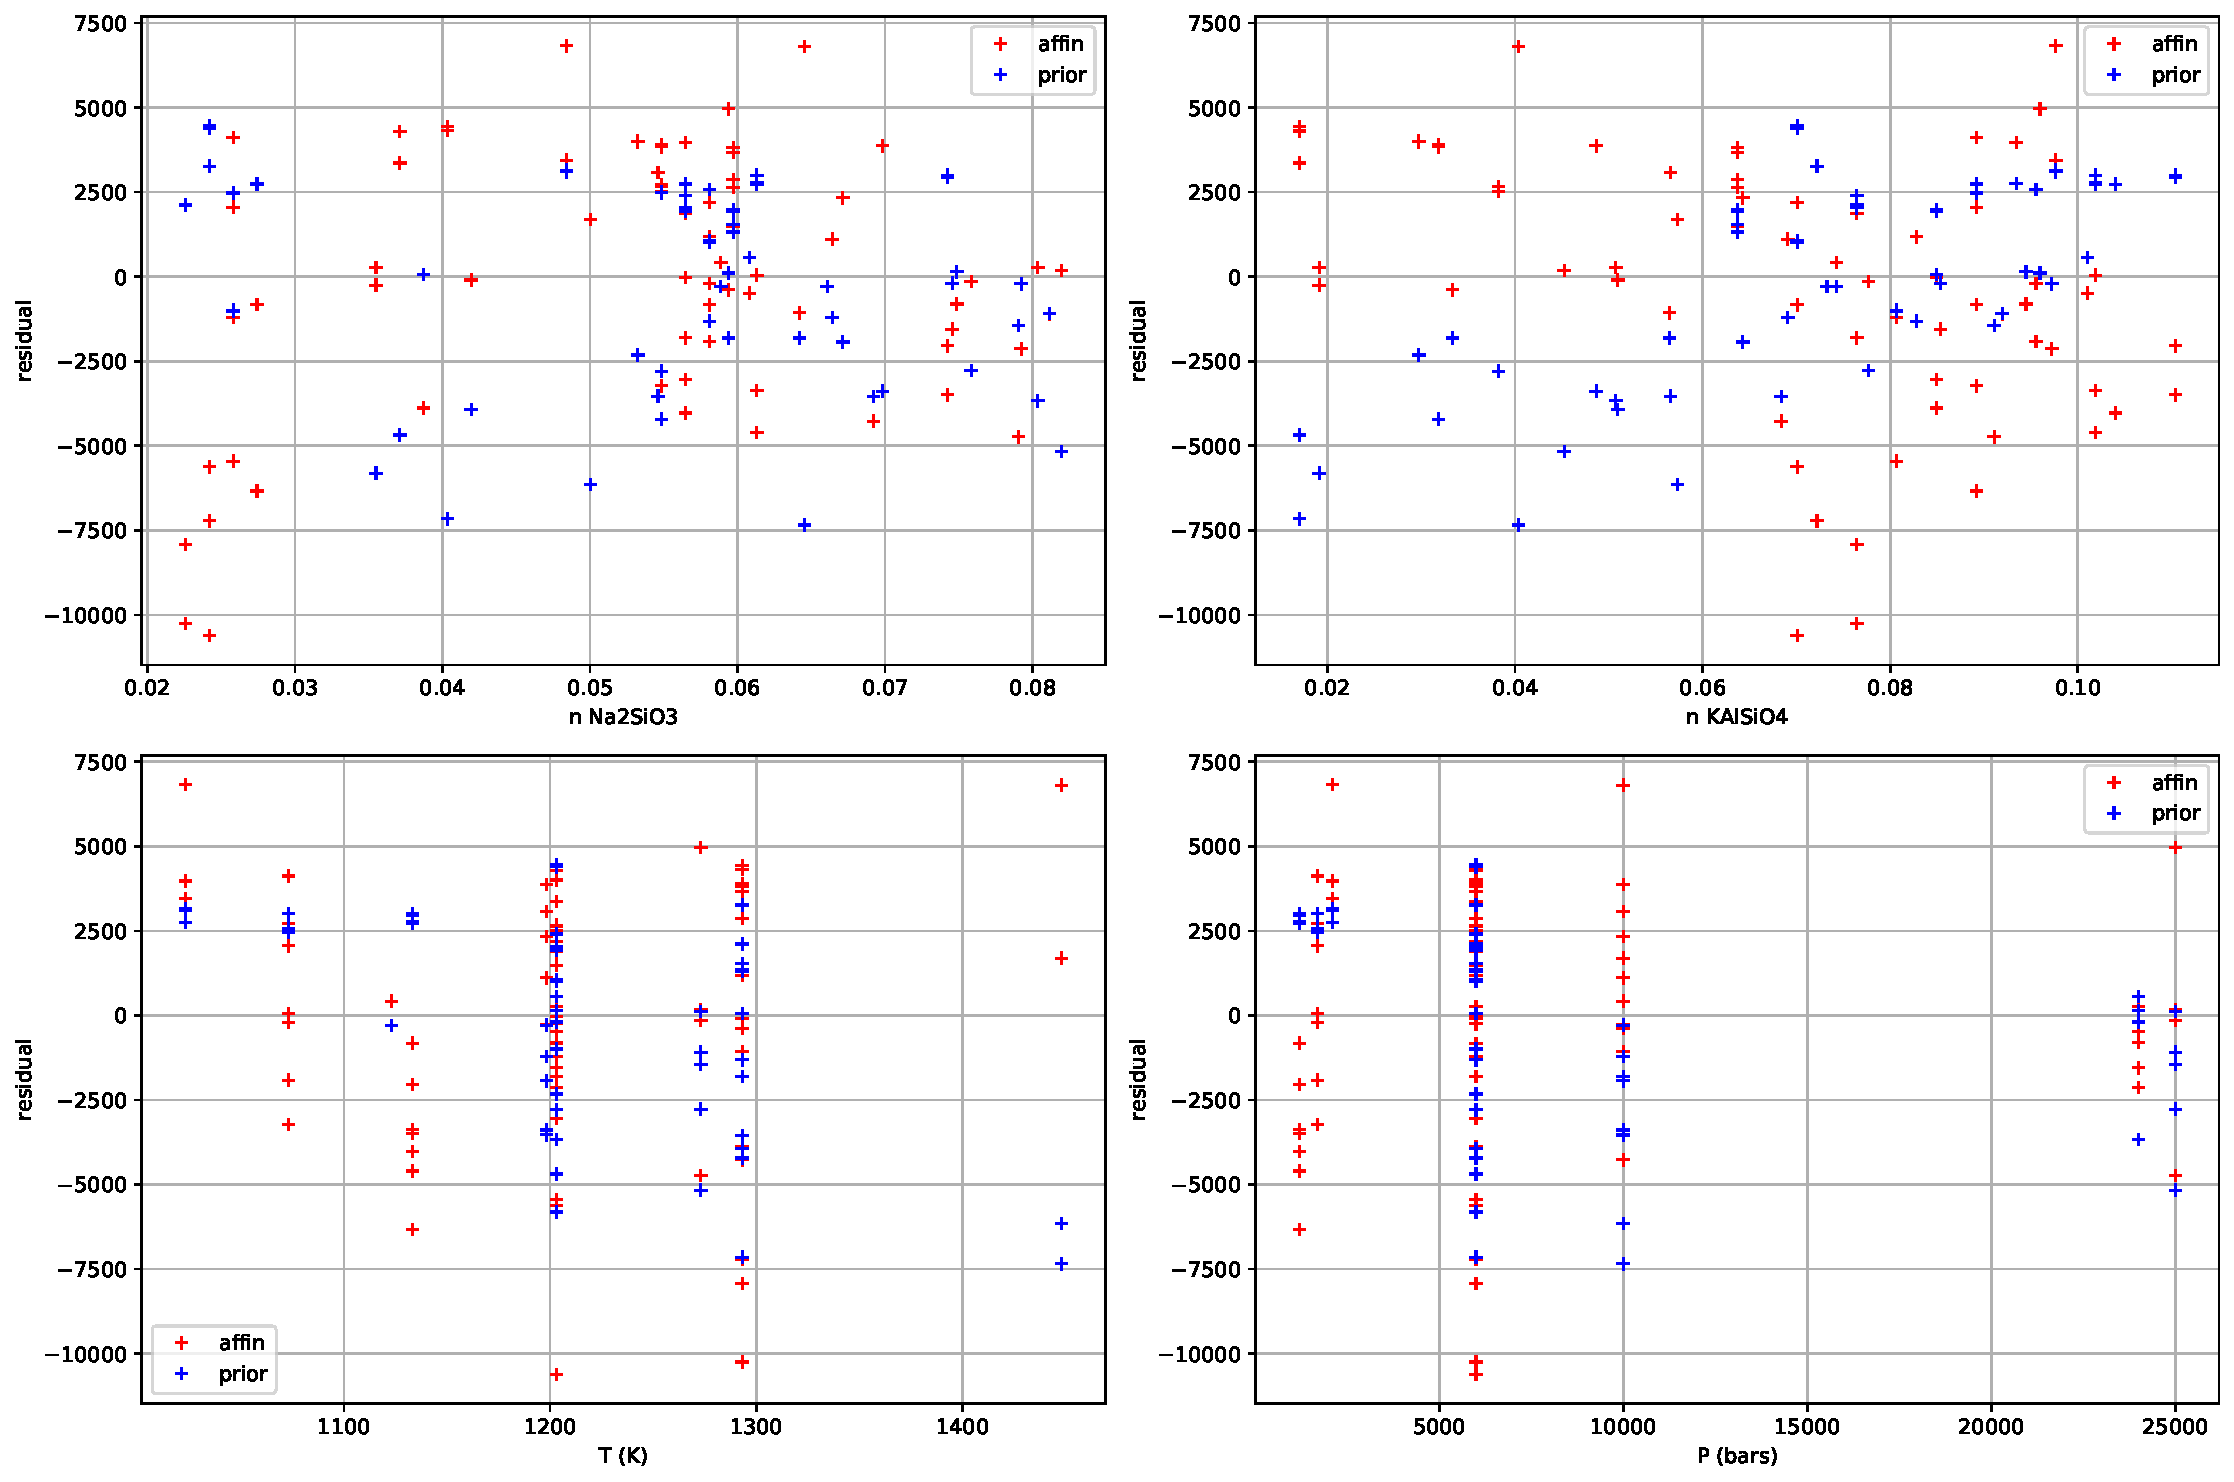
\includegraphics[width=1\textwidth,height=\textheight]{images/Figure_Residuals.pdf}

}

\caption{\label{fig-1}Model Residuals (J) plotted against (upper left)
sodium content of the liquid, as moles of Na2SiO3, (upper right)
potasssium content of the liquid, as moles of KAlSiO4, (lower left)
temperature (K), and (lower right) pressure (bars). Red crosses
correspond to residuals in the chemical affinity for the zircon
saturation reaction, and blue crosses correspond to residuals in the
Na/K logistic function utilized to inforce the prior that the ratio of
Na to K zirconate species abundance is strongly correlated to the
measured Na/K ratio in the liquid.}

\end{figure}%

\begin{figure}

\centering{

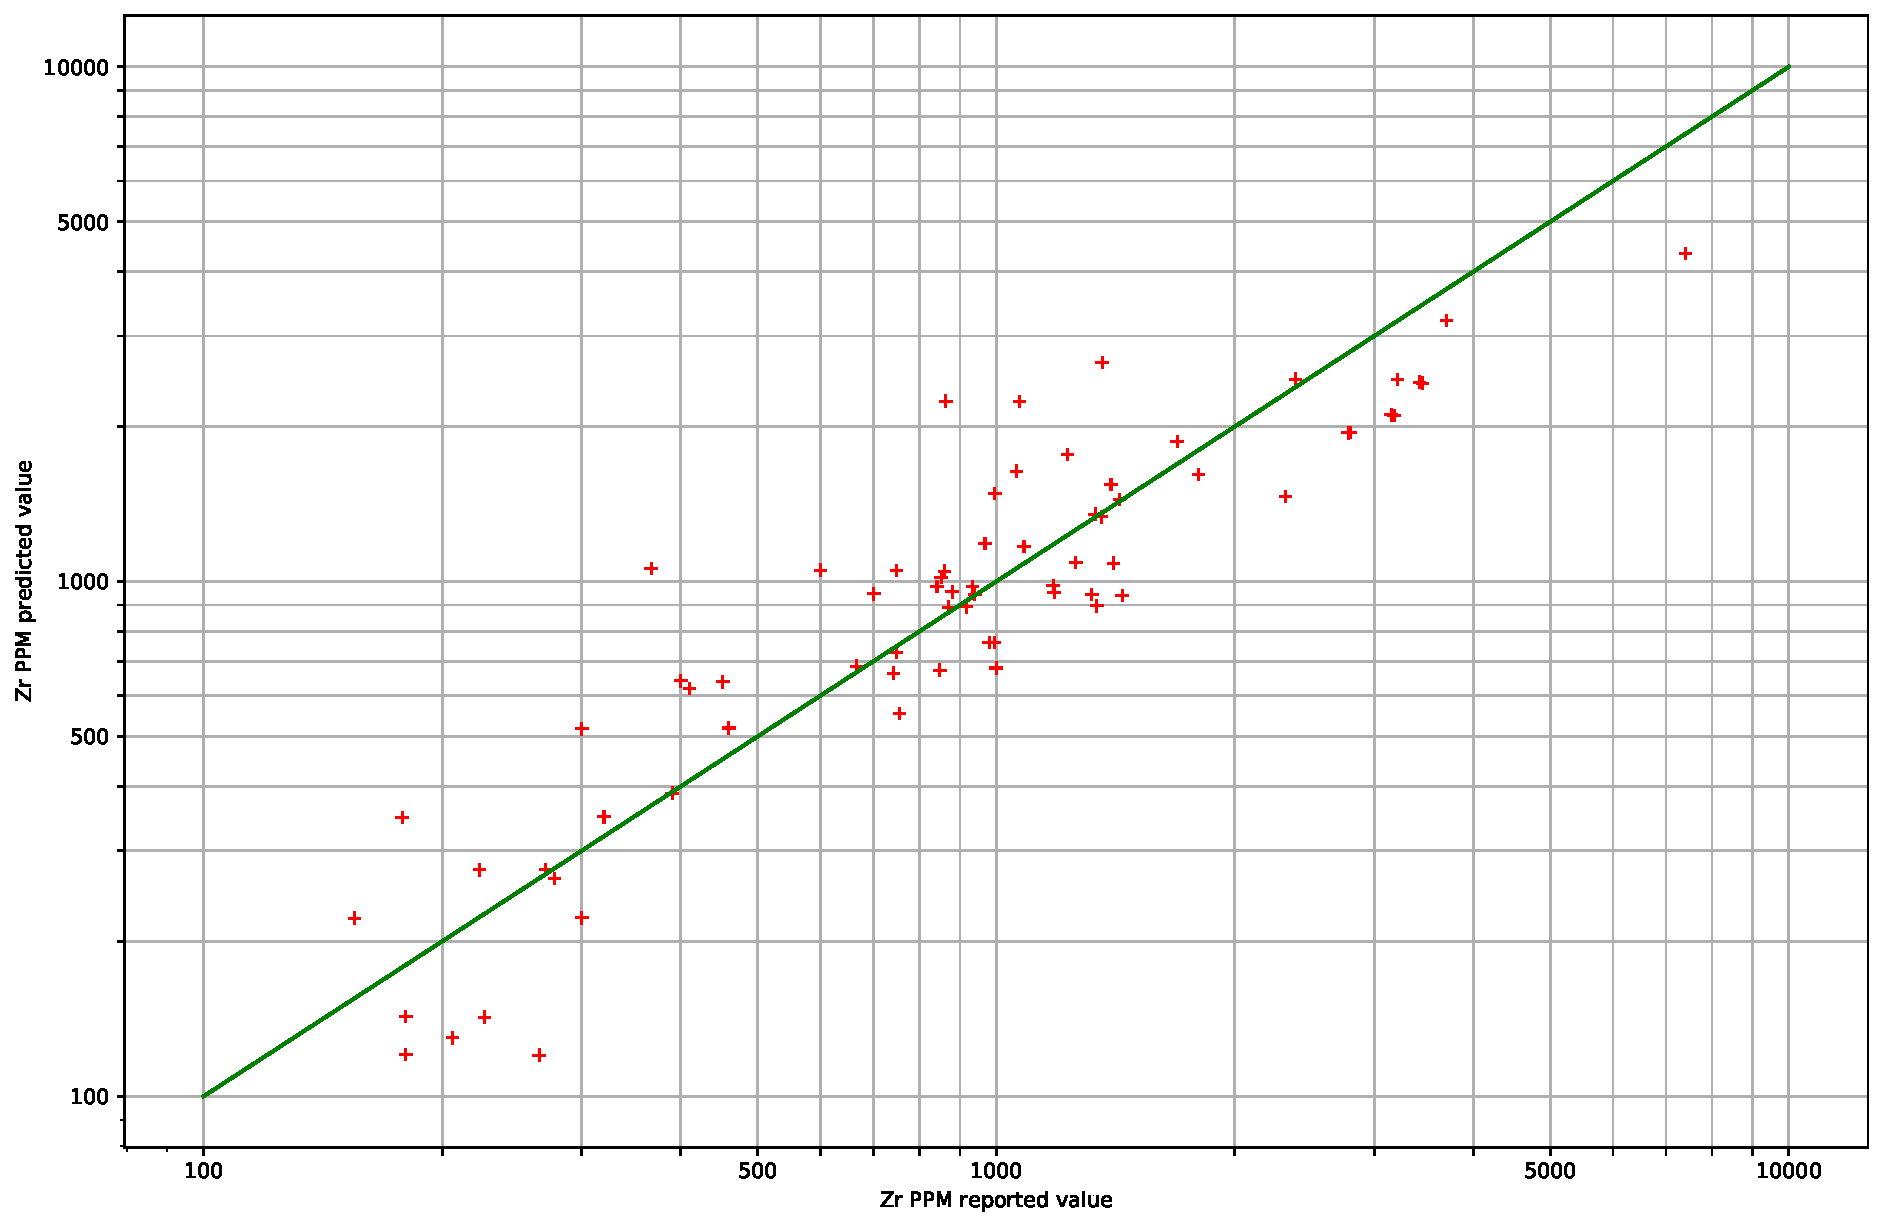
\includegraphics[width=1\textwidth,height=\textheight]{images/Figure_Zr_Zr.pdf}

}

\caption{\label{fig-2}Model Reported Zr concentrations (ordinate)
plotted against model estimate Zr concentrations (abscissa) for the
calibration data set. The estimate is constructed by finding the Zr
concentration that zeros the chemical affinity for zircon saturation in
the experimental liquid at fixed temperature and pressure.}

\end{figure}%

\begin{figure}

\centering{

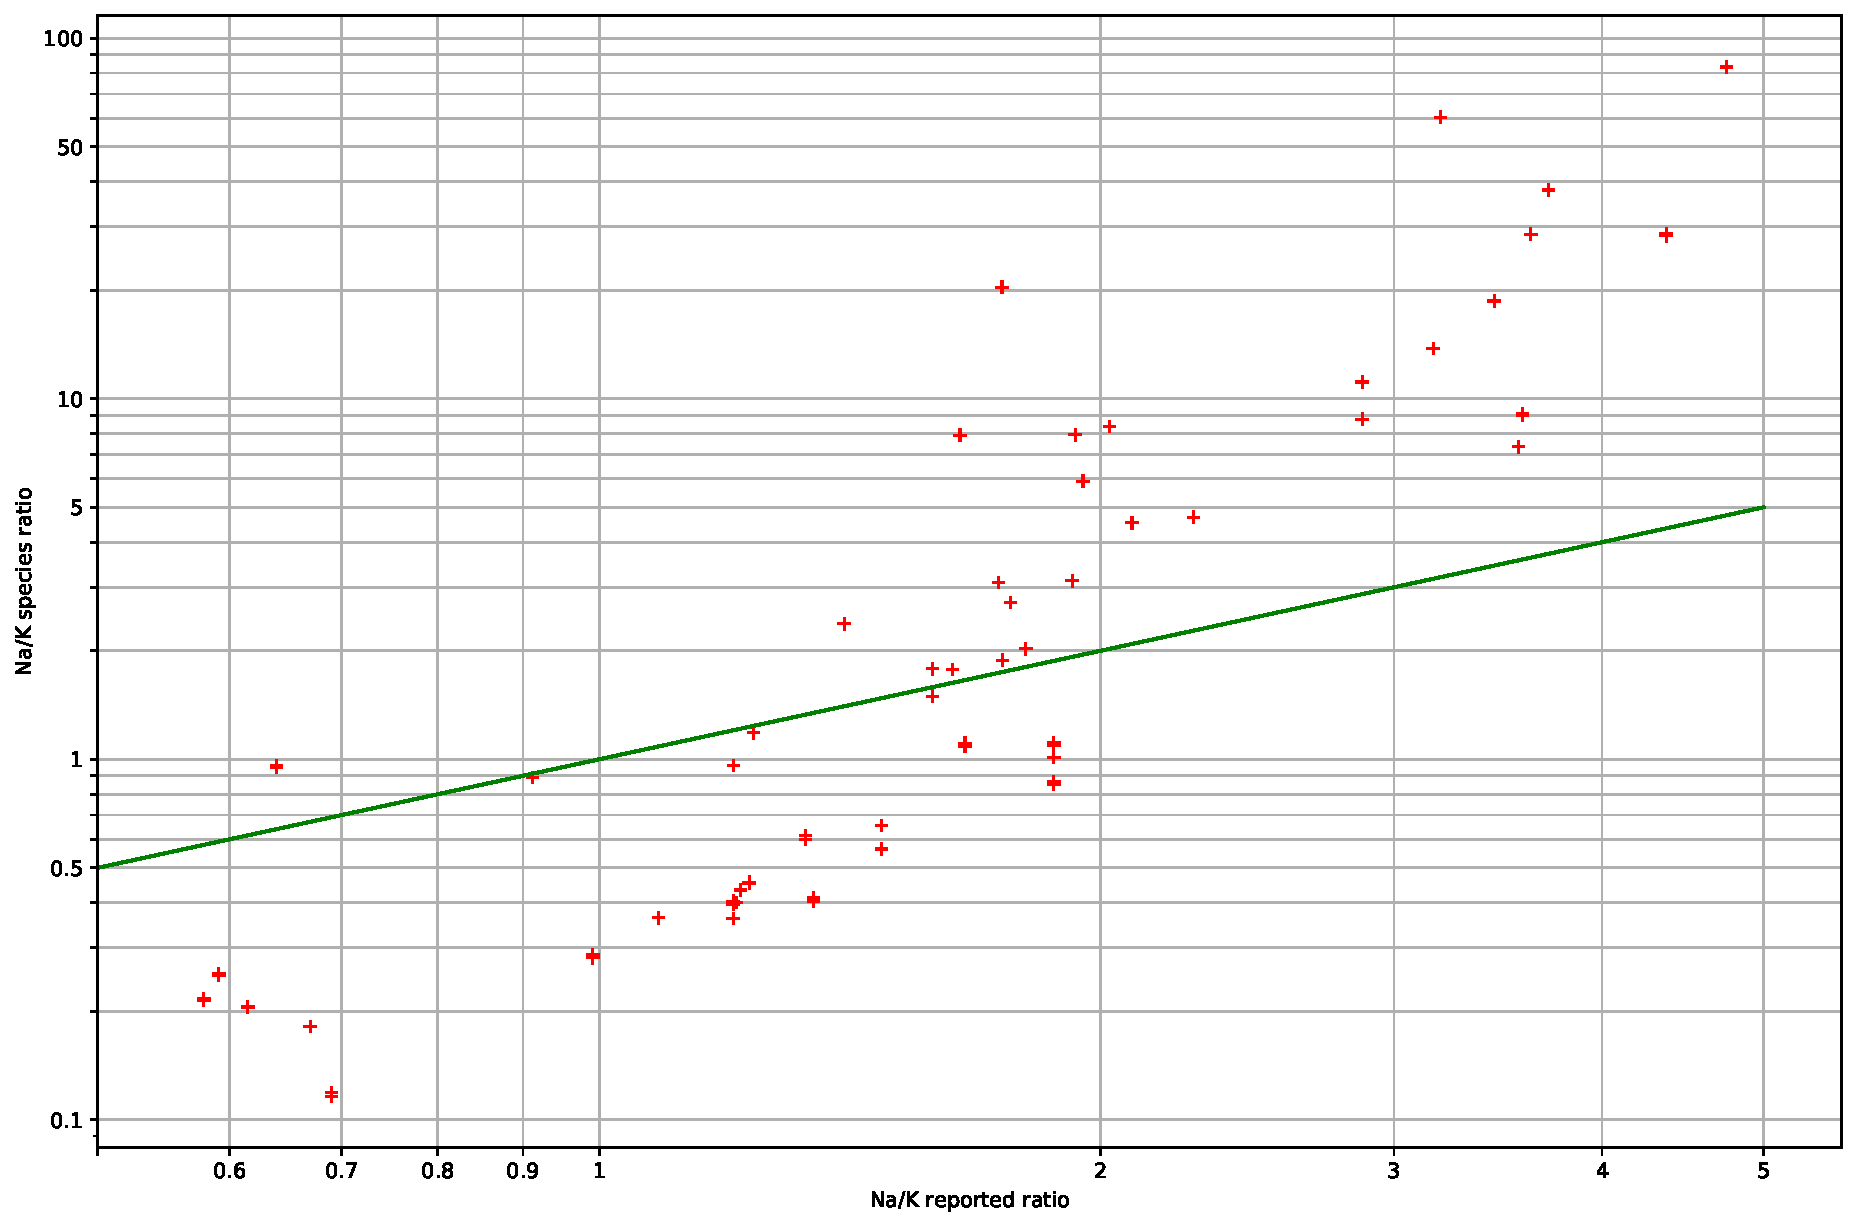
\includegraphics[width=1\textwidth,height=\textheight]{images/Figure_Na_K.pdf}

}

\caption{\label{fig-3}Model predicted Na/K ratios of alkali-zirconate
species in the liquid (abscissa) plotted against measured bulk Na/K
ratio in the liquid (ordinate). Green line refers to exact correlation.
This constraint is imposed as a logistic on model calibration. See
text.}

\end{figure}%

Quality of fit is evaluated in Figure~\ref{fig-1}, Figure~\ref{fig-2}
and Figure~\ref{fig-3}. Figure~\ref{fig-1} demonstrates that residuals
in zircon affinity show no correlation to alakli-content of the liquid,
nor to temperature and pressure. The lack of temperature and pressure
dependence of residuals supports our simplifying assumption that
\(\Delta S_{Na_4ZrSi_2O_8}\), \(\Delta S_{K_4ZrSi_2O_8}\),
\(\Delta S_{K_4ZrSi_2O_8}\), and \(\Delta V_{K_4ZrSi_2O_8}\) may be set
to zero. The absence of residual correlation to alkali-content implies
that alkli-zirconate speciation accounts for the alkali-effect on the
``effective-concentration'' (i.e., the activity) of ZrSiO4 in
alkali-rich liquids. Figure~\ref{fig-2} demonstrates recovery of Zr
liquid concentration, calculated by adjusting liquid Zr-content in order
to zero zircon affinity, plotted against measured values. Estimated Zr
concentrations scatter about a 1:1 line plotted against reported
concentrations. There is no systematic change in scatter of predicted
versus measured value as a function of Zr-concentration over two orders
of magnitude. Figure~\ref{fig-3} illustrates recovery of priors
residuals for the regression data set. While priors residuals are small
(fall close to the green line) for typical Na/K melt ratios, there is
significant deviation at elevated Na/K. The consequences of these
deviations may effect recovery of zircon phase relations in phonolitic
or pantelleritic composition melts with high Na/K, and this isue will be
further examined below.

\section{Discussion}\label{discussion}

The model calibrated above is evaluated in this section by constructing
zircon saturation curves for a variety of natural magma types and by
examing zircon saturation in conjunction with phase equilibrium
calculations using an augmented rhyolite-MELTS model.

\begin{longtable}[]{@{}
  >{\raggedright\arraybackslash}p{(\columnwidth - 20\tabcolsep) * \real{0.0909}}
  >{\raggedright\arraybackslash}p{(\columnwidth - 20\tabcolsep) * \real{0.0909}}
  >{\raggedright\arraybackslash}p{(\columnwidth - 20\tabcolsep) * \real{0.0909}}
  >{\raggedright\arraybackslash}p{(\columnwidth - 20\tabcolsep) * \real{0.0909}}
  >{\raggedright\arraybackslash}p{(\columnwidth - 20\tabcolsep) * \real{0.0909}}
  >{\raggedright\arraybackslash}p{(\columnwidth - 20\tabcolsep) * \real{0.0909}}
  >{\raggedright\arraybackslash}p{(\columnwidth - 20\tabcolsep) * \real{0.0909}}
  >{\raggedright\arraybackslash}p{(\columnwidth - 20\tabcolsep) * \real{0.0909}}
  >{\raggedright\arraybackslash}p{(\columnwidth - 20\tabcolsep) * \real{0.0909}}
  >{\raggedright\arraybackslash}p{(\columnwidth - 20\tabcolsep) * \real{0.0909}}
  >{\raggedright\arraybackslash}p{(\columnwidth - 20\tabcolsep) * \real{0.0909}}@{}}
\caption{Bulk compositions of lavas (wt\%): {[}1{]} Carmichael et al.
(1974), {[}2{]} Lowenstern \& Mahood (1991), {[}3{]} Gualda et al.
(2012), {[}4{]} Carmichael (1967), Madupite is LH.16 and contains
appreciable wadeite, Zr2K4Si6O18. This rock has 0.27 wt\% ZrO2. The
Wyomingite is LH.3. The rock has no Zr analysis but other wyomingites
have 0.28 wt\% ZrO2. All the analyses are from Table 12 (page
50)}\label{tbl-4}\tabularnewline
\toprule\noalign{}
\begin{minipage}[b]{\linewidth}\raggedright
\end{minipage} & \begin{minipage}[b]{\linewidth}\raggedright
High-silica rhyolite
\end{minipage} & \begin{minipage}[b]{\linewidth}\raggedright
Iceland rhyolite
\end{minipage} & \begin{minipage}[b]{\linewidth}\raggedright
California rhyolite
\end{minipage} & \begin{minipage}[b]{\linewidth}\raggedright
dacite
\end{minipage} & \begin{minipage}[b]{\linewidth}\raggedright
pantellerite
\end{minipage} & \begin{minipage}[b]{\linewidth}\raggedright
comendite
\end{minipage} & \begin{minipage}[b]{\linewidth}\raggedright
trachyte
\end{minipage} & \begin{minipage}[b]{\linewidth}\raggedright
phonolite
\end{minipage} & \begin{minipage}[b]{\linewidth}\raggedright
madupite
\end{minipage} & \begin{minipage}[b]{\linewidth}\raggedright
wyomingite
\end{minipage} \\
\midrule\noalign{}
\endfirsthead
\toprule\noalign{}
\begin{minipage}[b]{\linewidth}\raggedright
\end{minipage} & \begin{minipage}[b]{\linewidth}\raggedright
High-silica rhyolite
\end{minipage} & \begin{minipage}[b]{\linewidth}\raggedright
Iceland rhyolite
\end{minipage} & \begin{minipage}[b]{\linewidth}\raggedright
California rhyolite
\end{minipage} & \begin{minipage}[b]{\linewidth}\raggedright
dacite
\end{minipage} & \begin{minipage}[b]{\linewidth}\raggedright
pantellerite
\end{minipage} & \begin{minipage}[b]{\linewidth}\raggedright
comendite
\end{minipage} & \begin{minipage}[b]{\linewidth}\raggedright
trachyte
\end{minipage} & \begin{minipage}[b]{\linewidth}\raggedright
phonolite
\end{minipage} & \begin{minipage}[b]{\linewidth}\raggedright
madupite
\end{minipage} & \begin{minipage}[b]{\linewidth}\raggedright
wyomingite
\end{minipage} \\
\midrule\noalign{}
\endhead
\bottomrule\noalign{}
\endlastfoot
& {[}3{]} & {[}1{]} & {[}1{]} & {[}1{]} & {[}1{]},{[}2{]} & {[}1{]} &
{[}1{]} & {[}1{]} & {[}4{]} & {[}4{]} \\
SiO2 & 77.5 & 74.96 & 75.04 & 63.58 & 69.81 & 73.06 & 57.73 & 54.55 &
43.56 & 50.23 \\
TiO2 & 0.08 & 0.23 & 0.07 & 0.64 & 0.45 & 0.23 & 1.18 & 1.60 & 2.31 &
2.27 \\
Al2O3 & 12.5 & 12.55 & 12.29 & 16.67 & 8.59 & 9.76 & 17.05 & 19.00 &
7.85 & 11.22 \\
Fe2O3 & 0.207 & 1.72 & 0.33 & 2.24 & 2.28 & 2.74 & 2.55 & 1.75 & 5.57 &
3.34 \\
Cr2O3 & - & - & - & - & - & - & - & - & 0.04 & - \\
FeO & 0.473 & 0.71 & 0.71 & 3.00 & 5.76 & 2.70 & 4.35 & 3.78 & 0.85 &
1.84 \\
MnO & - & 0.04 & 0.05 & 0.11 & 0.28 & 0.13 & 0.28 & 0.16 & 0.15 &
0.05 \\
MgO & 0.03 & 0.02 & 0.04 & 2.12 & 0.10 & 0.10 & 1.11 & 1.76 & 11.03 &
7.09 \\
CaO & 0.43 & 0.90 & 0.58 & 5.53 & 0.42 & 0.32 & 3.10 & 4.07 & 11.89 &
5.99 \\
Na2O & 3.98 & 4.41 & 4.03 & 3.98 & 6.46 & 5.64 & 6.81 & 9.06 & 0.74 &
1.37 \\
K2O & 4.88 & 3.65 & 4.66 & 1.40 & 4.49 & 4.34 & 4.27 & 3.64 & 7.19 &
9.81 \\
P2O5 & - & 0.04 & 0.01 & - & - & 0.02 & 0.34 & 0.20 & 1.50 & 1.89 \\
H2O & 5.5 & 5.5 & 5.5 & 3.00 & 2.5 & 2.5 & 1.0 & 1.0 & 1.0 & 2.0 \\
CO2 & 0.05 & 0.05 & 0.05 & 0.05 & 0.05 & 0.05 & 0.05 & 0.05 & 0.05 &
0.05 \\
Zr PPM & 100 & 385 & - & 150 & 1800 & - & - & - & 2073 & 2073 \\
\end{longtable}

\subsection{Zircon Saturation Curves}\label{zircon-saturation-curves}

Bulk compositions of a wide variety of silicic magma types are listed in
Table~\ref{tbl-4}. This tabulation includes determinations of Zr
concentration. Bulk compositions listed in the first four columns of
Table~\ref{tbl-4} are likely zircon saturated, whereas magma types
listed in columns five through ten are not associated with a zircon
solid phase. The madupite and wyomingite represent extreme compositions
and are saturated with the zirconium-bearing mineral wadeite,
Zr2K4Si6O18, which forms in lieu of zircon in these rocks.

\begin{figure}

\begin{minipage}{\linewidth}

\centering{

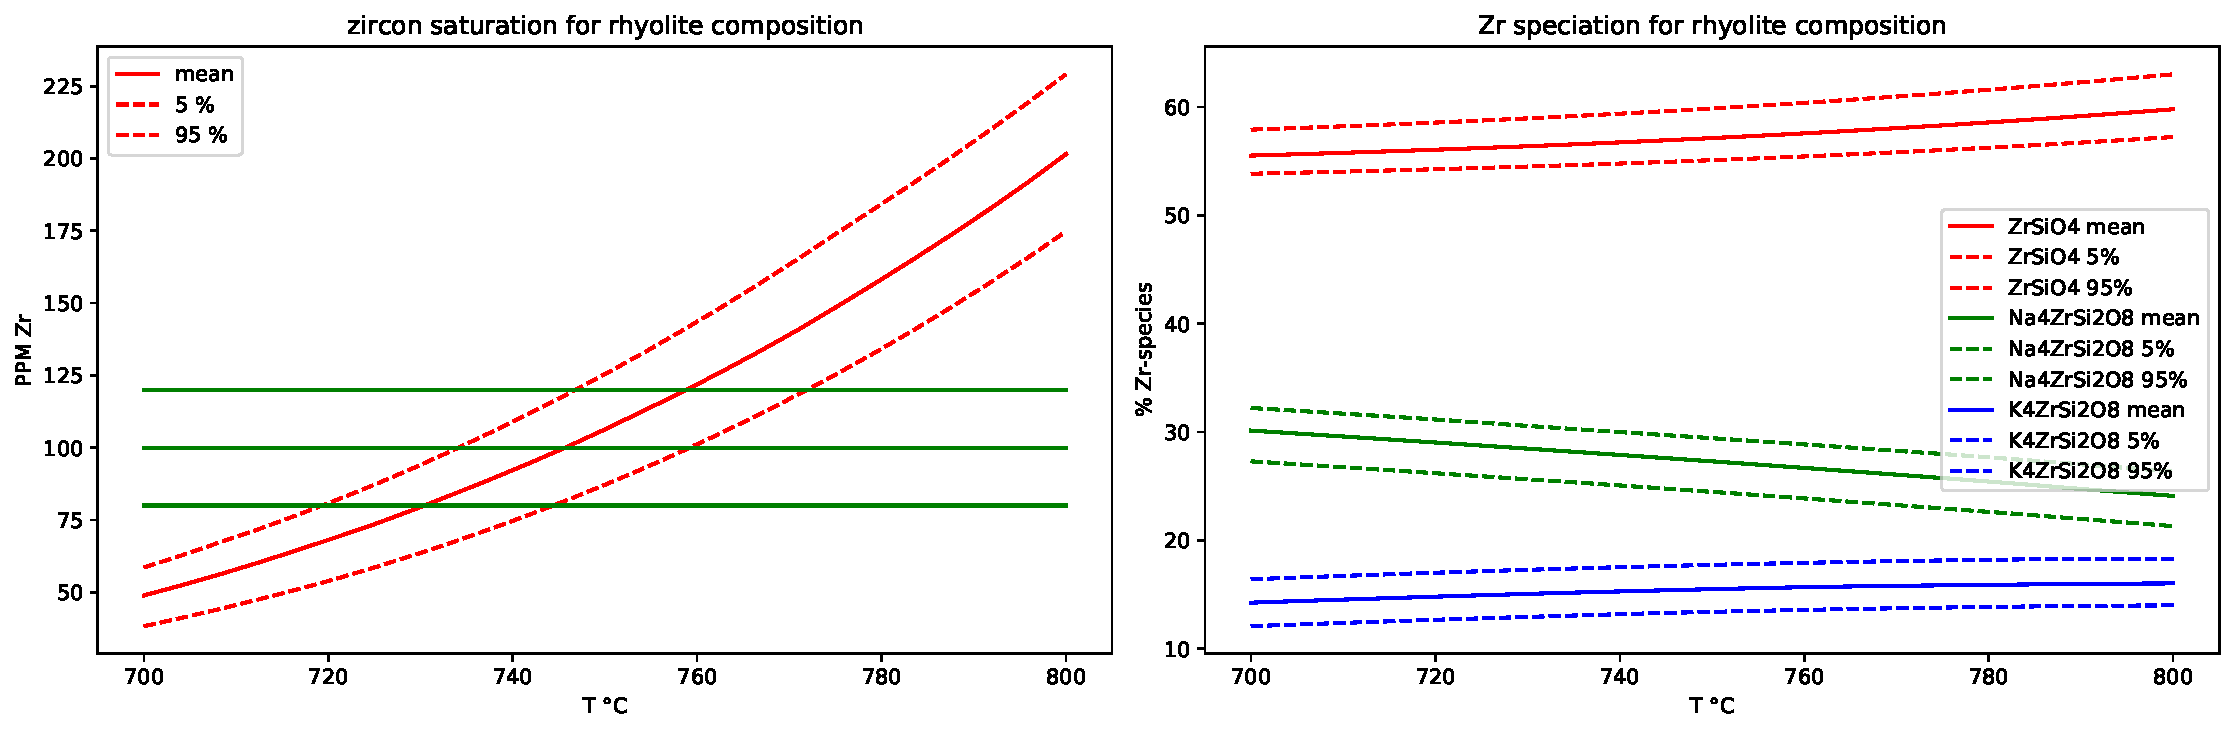
\includegraphics{images/zircon_sat_rhyolite.pdf}

}

\subcaption{\label{fig-4a}High-silica rhyolite}

\end{minipage}%
\newline
\begin{minipage}{\linewidth}

\centering{

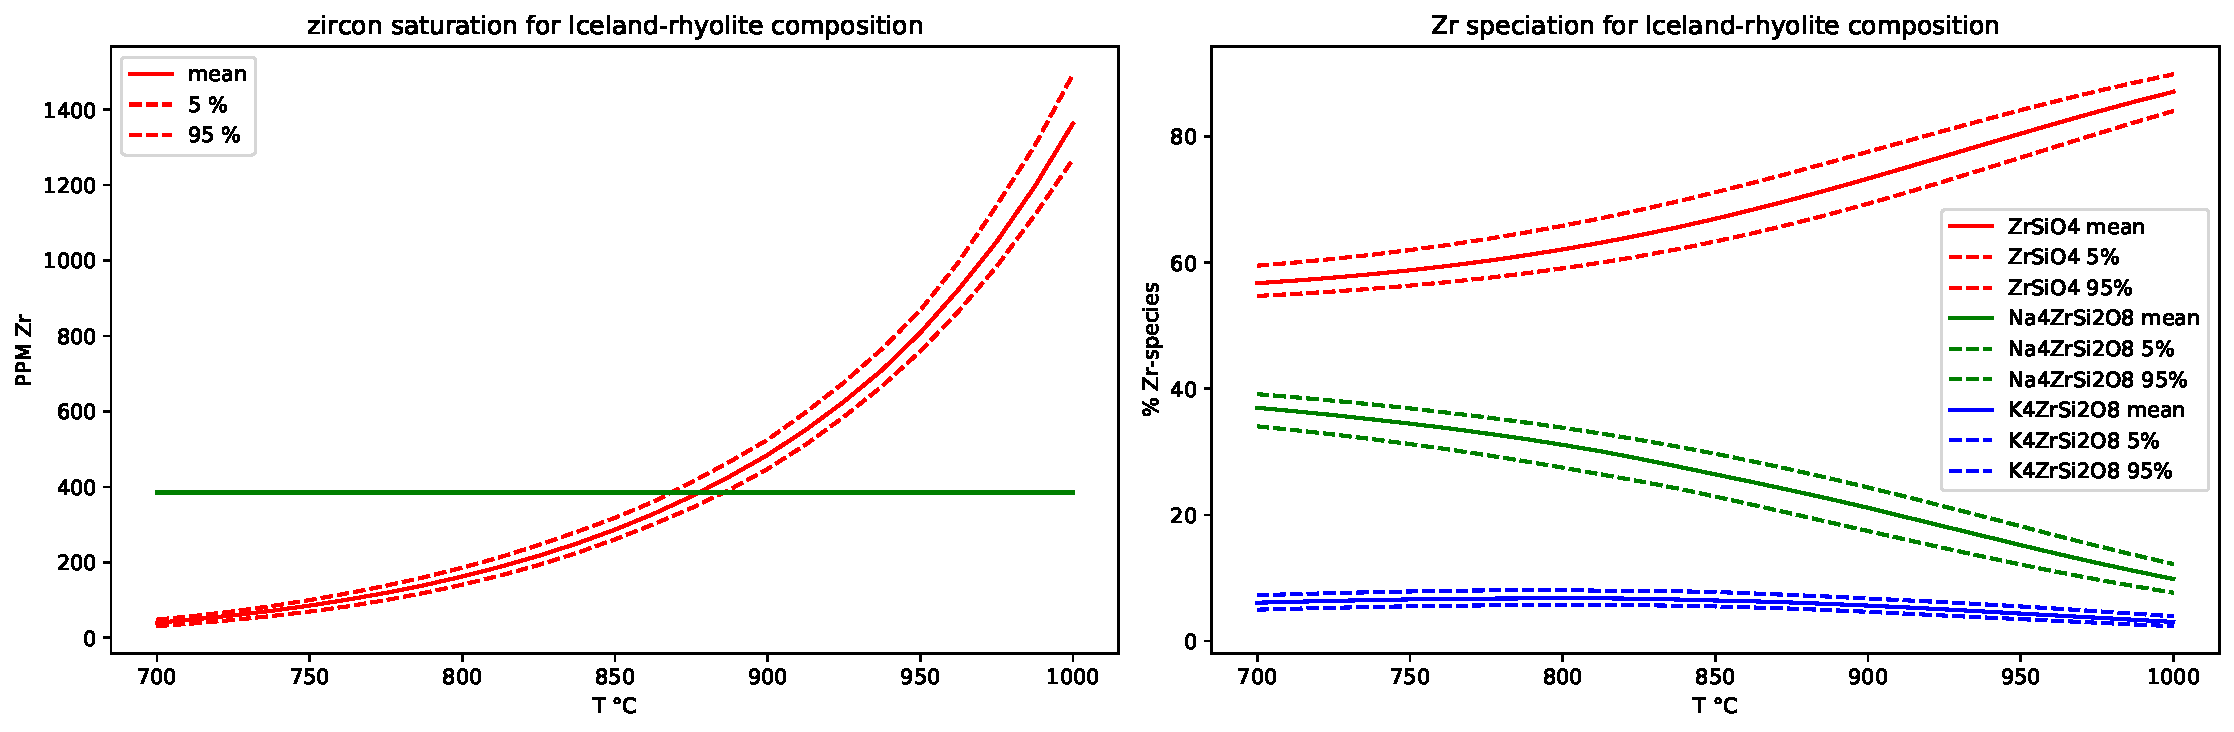
\includegraphics{images/zircon_sat_Iceland-rhyolite.pdf}

}

\subcaption{\label{fig-4b}Icelandic rhyolite}

\end{minipage}%
\newline
\begin{minipage}{\linewidth}

\centering{

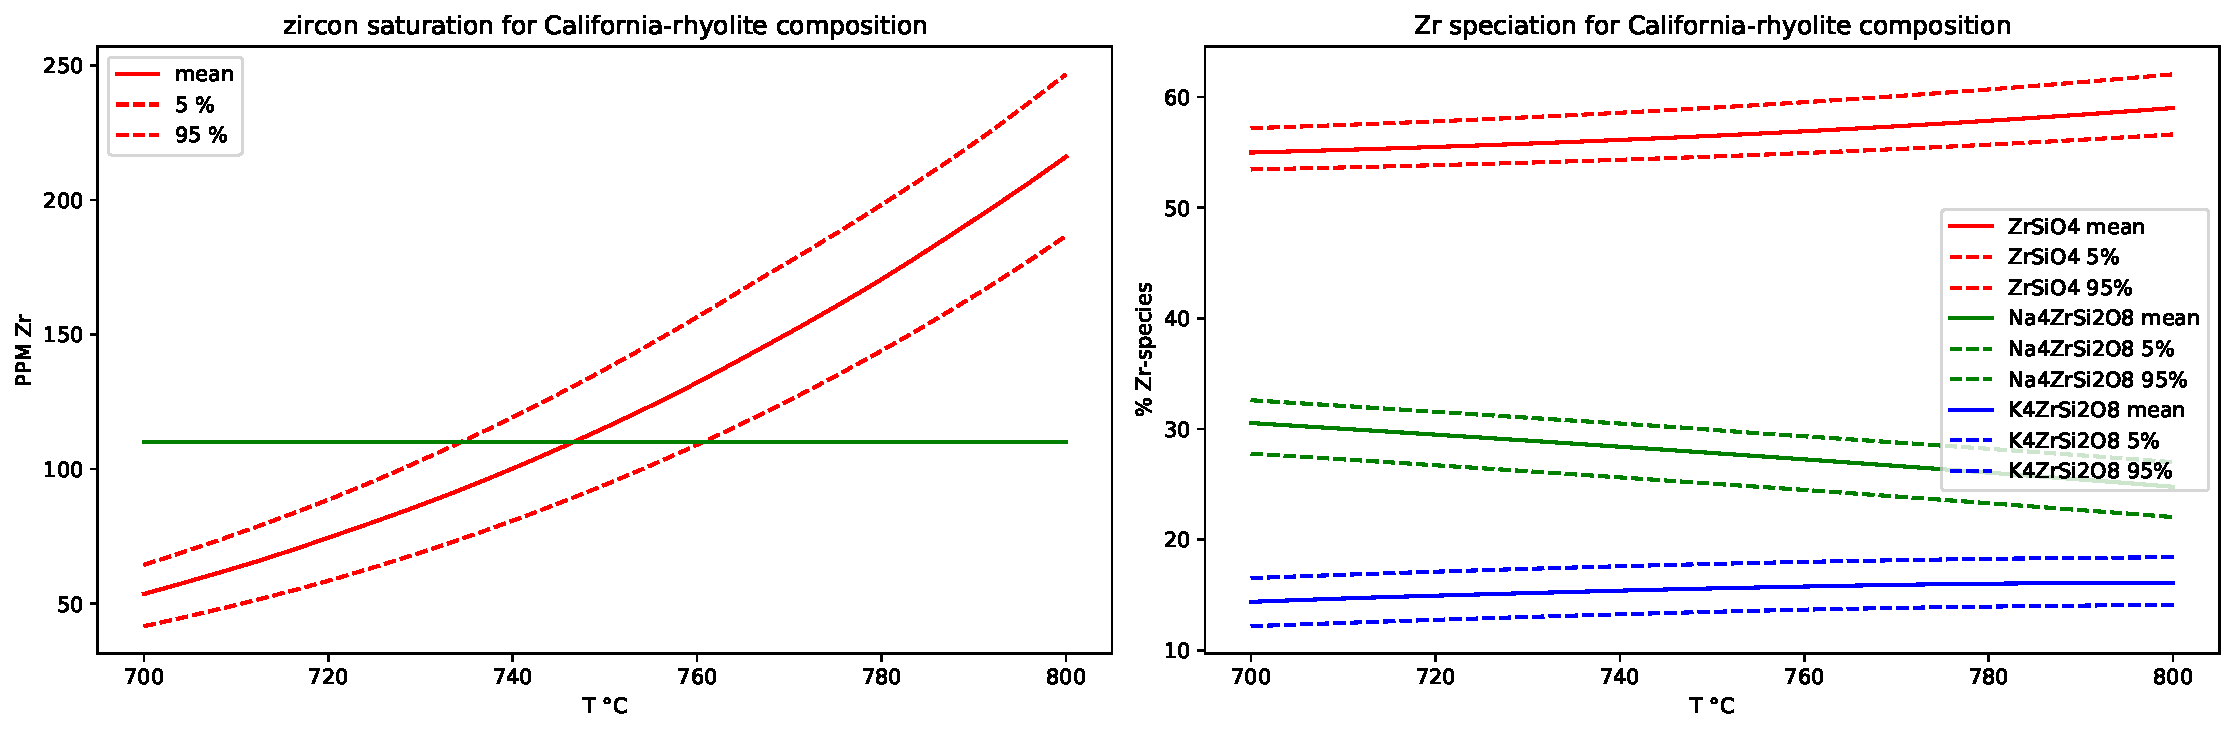
\includegraphics{images/zircon_sat_California-rhyolite.pdf}

}

\subcaption{\label{fig-4c}California rhyolite}

\end{minipage}%
\newline
\begin{minipage}{\linewidth}

\centering{

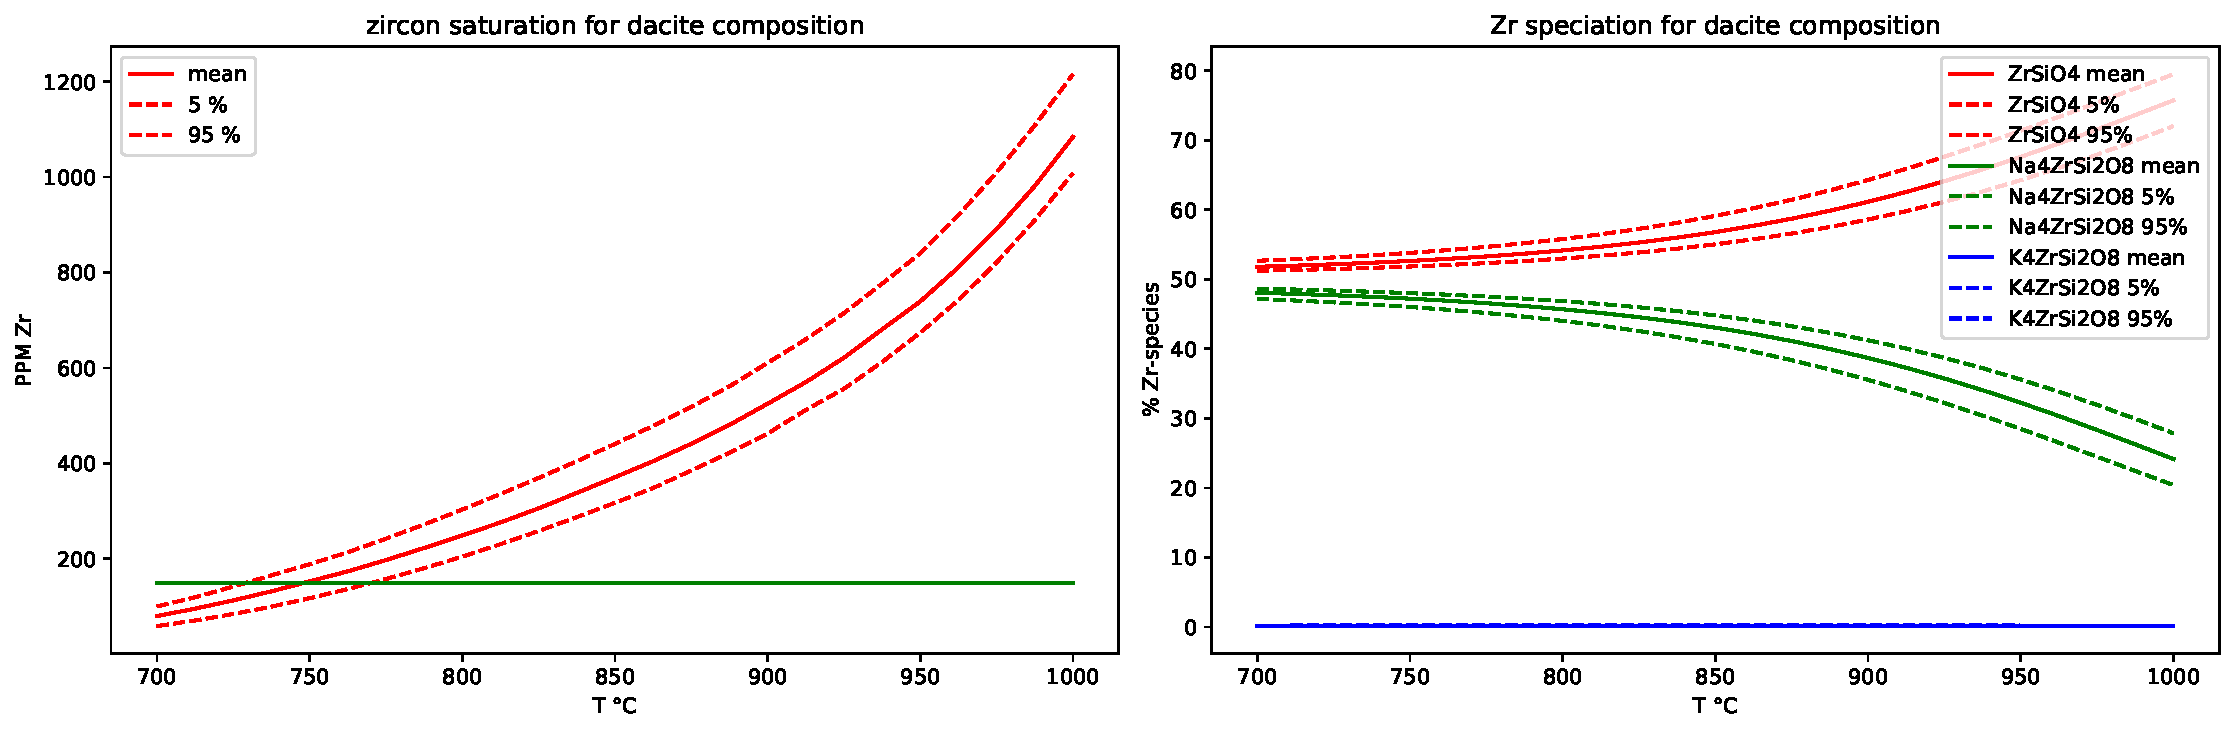
\includegraphics{images/zircon_sat_dacite.pdf}

}

\subcaption{\label{fig-4d}Dacite}

\end{minipage}%
\newline
\begin{minipage}{\linewidth}

\centering{

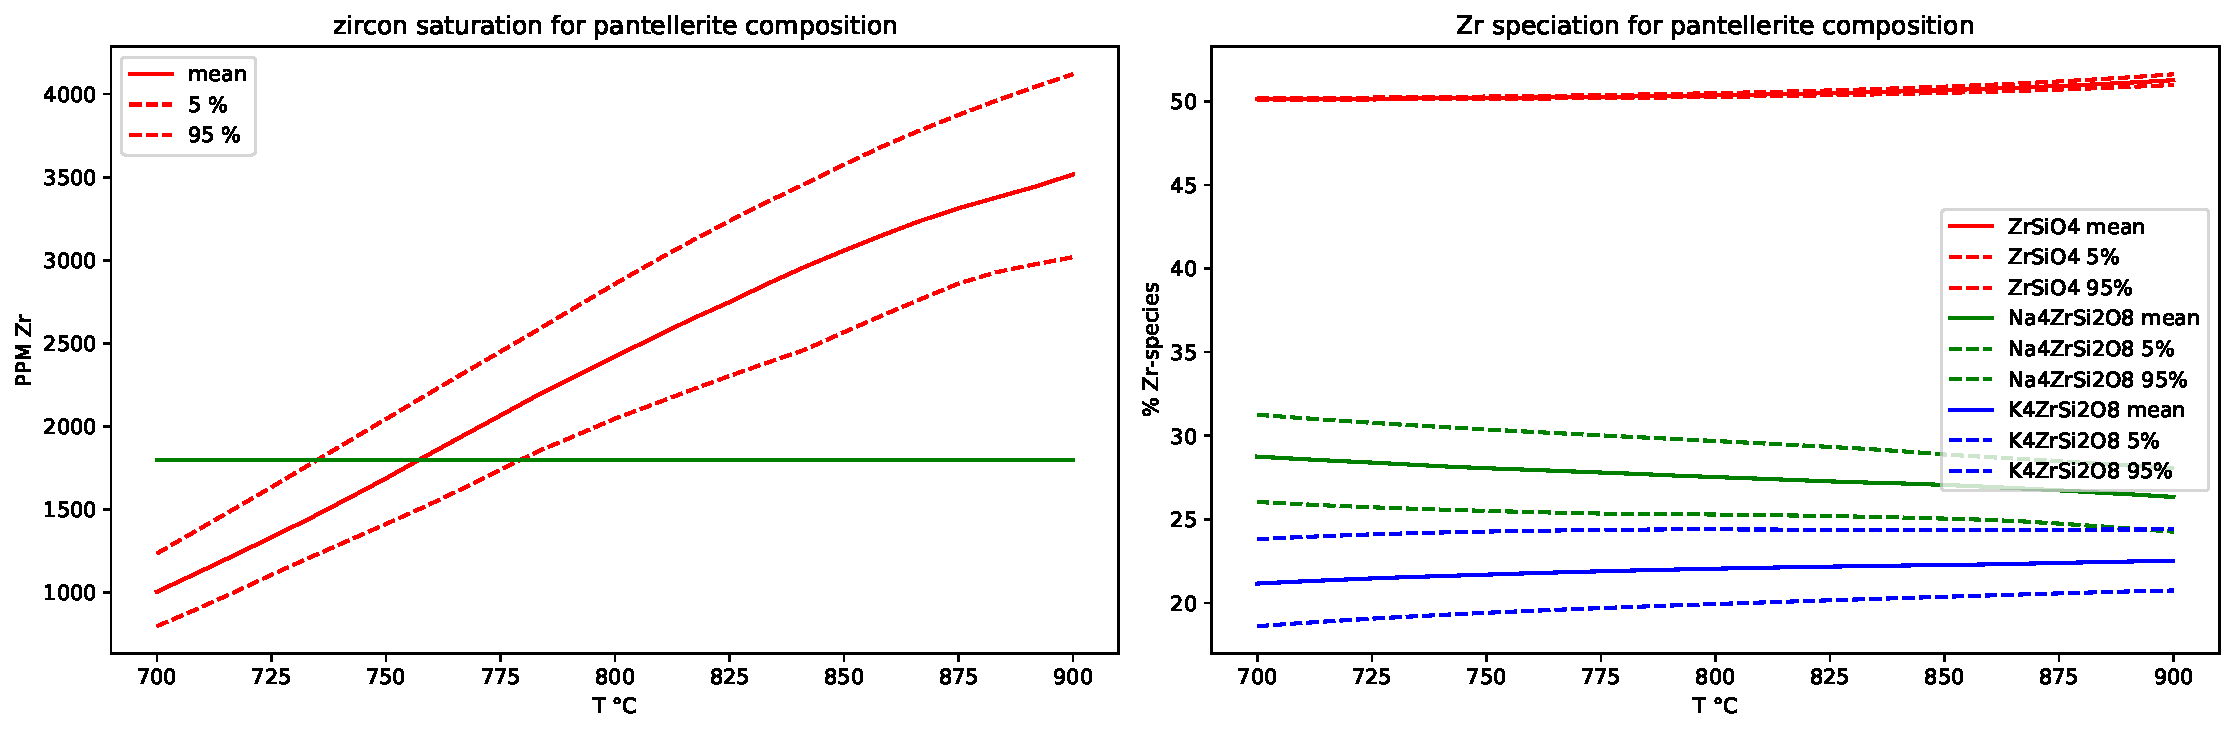
\includegraphics{images/zircon_sat_pantellerite.pdf}

}

\subcaption{\label{fig-4e}Pantellerite}

\end{minipage}%
\newline
\begin{minipage}{\linewidth}

\centering{

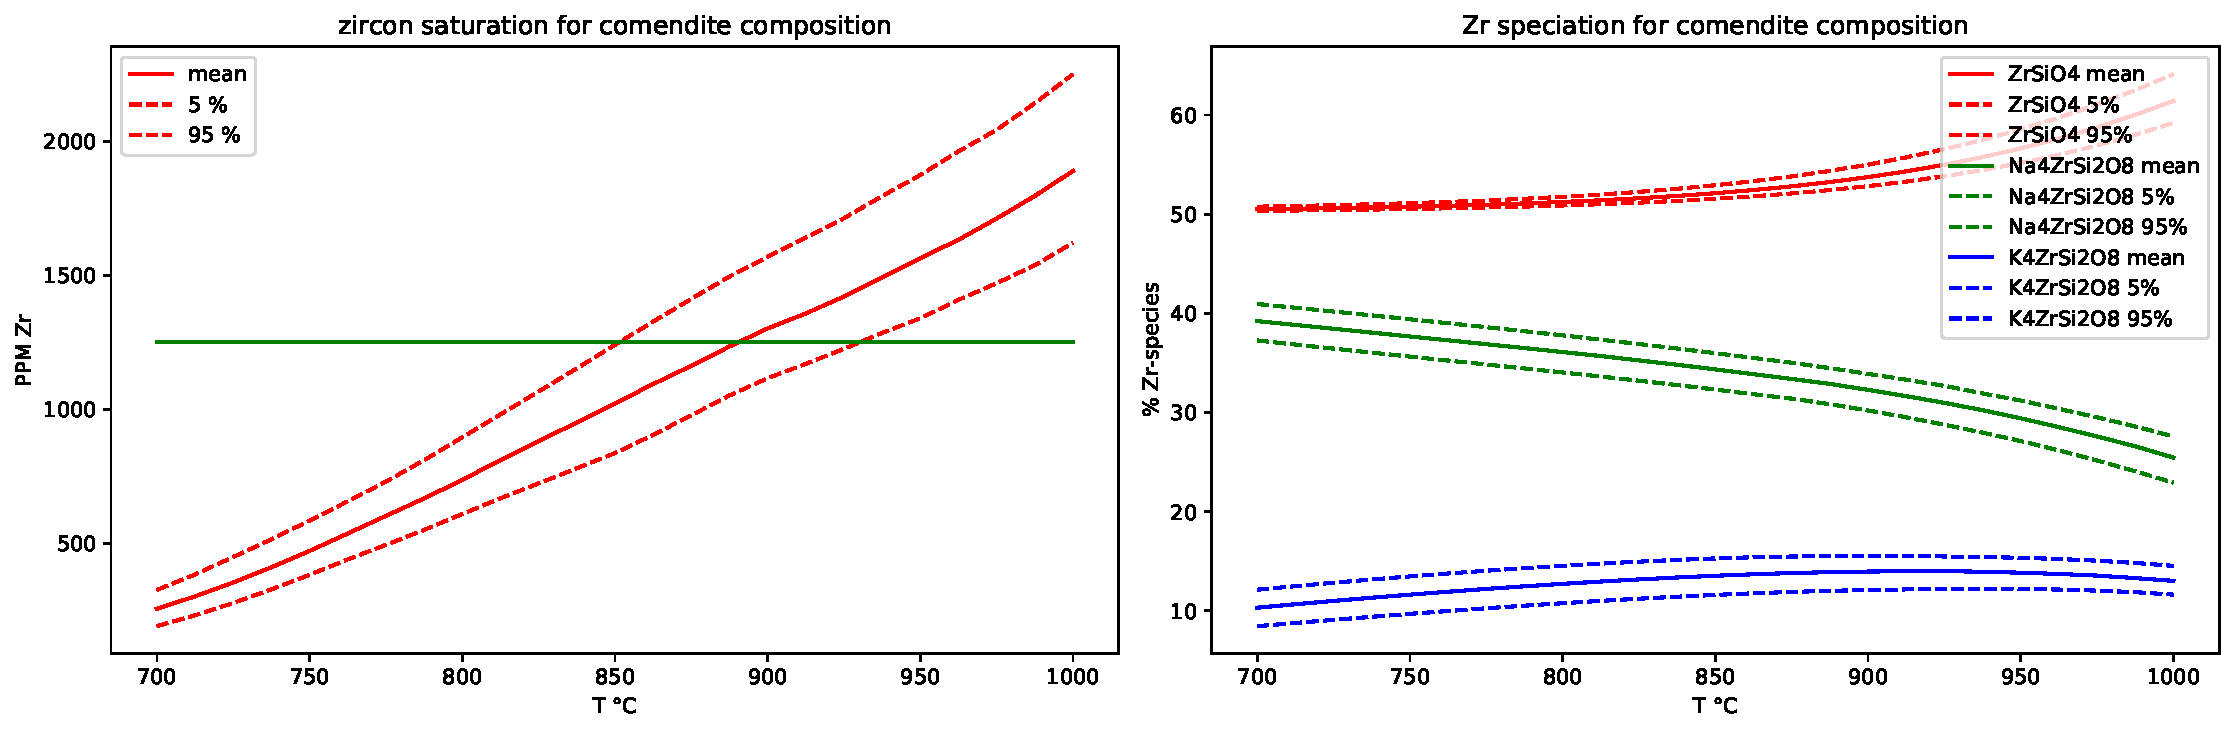
\includegraphics{images/zircon_sat_comendite.pdf}

}

\subcaption{\label{fig-4f}Comendite}

\end{minipage}%
\newline
\begin{minipage}{\linewidth}

\centering{

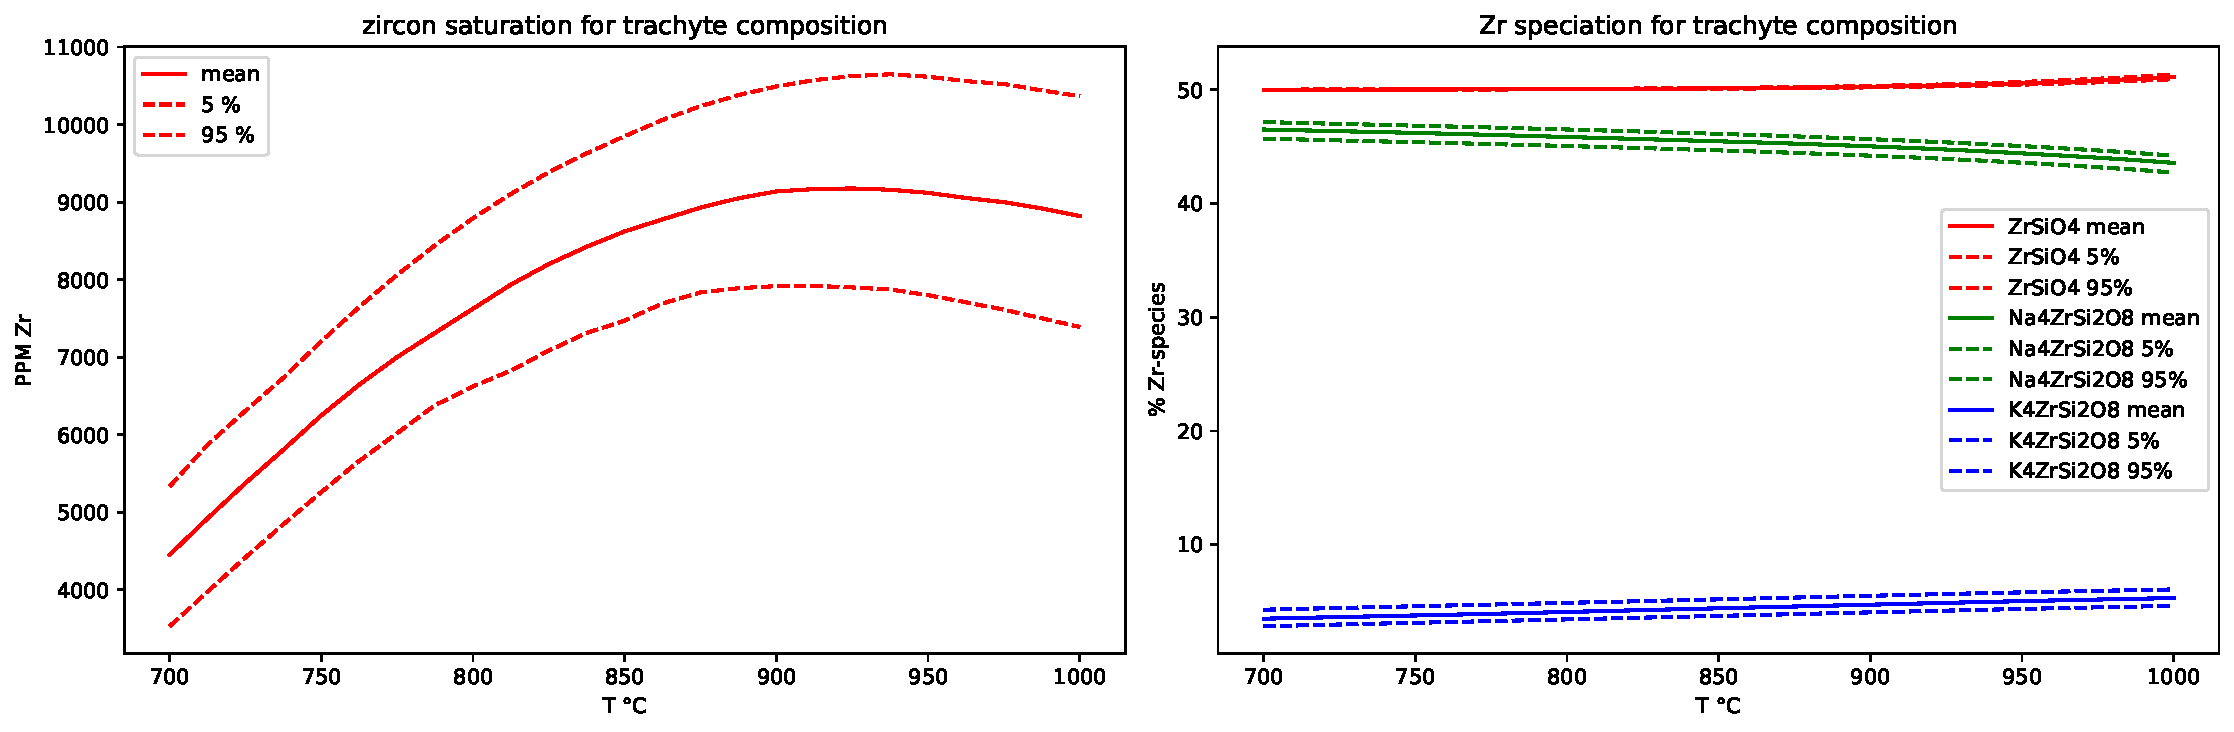
\includegraphics{images/zircon_sat_trachyte.pdf}

}

\subcaption{\label{fig-4g}Trachyte}

\end{minipage}%
\newline
\begin{minipage}{\linewidth}

\centering{

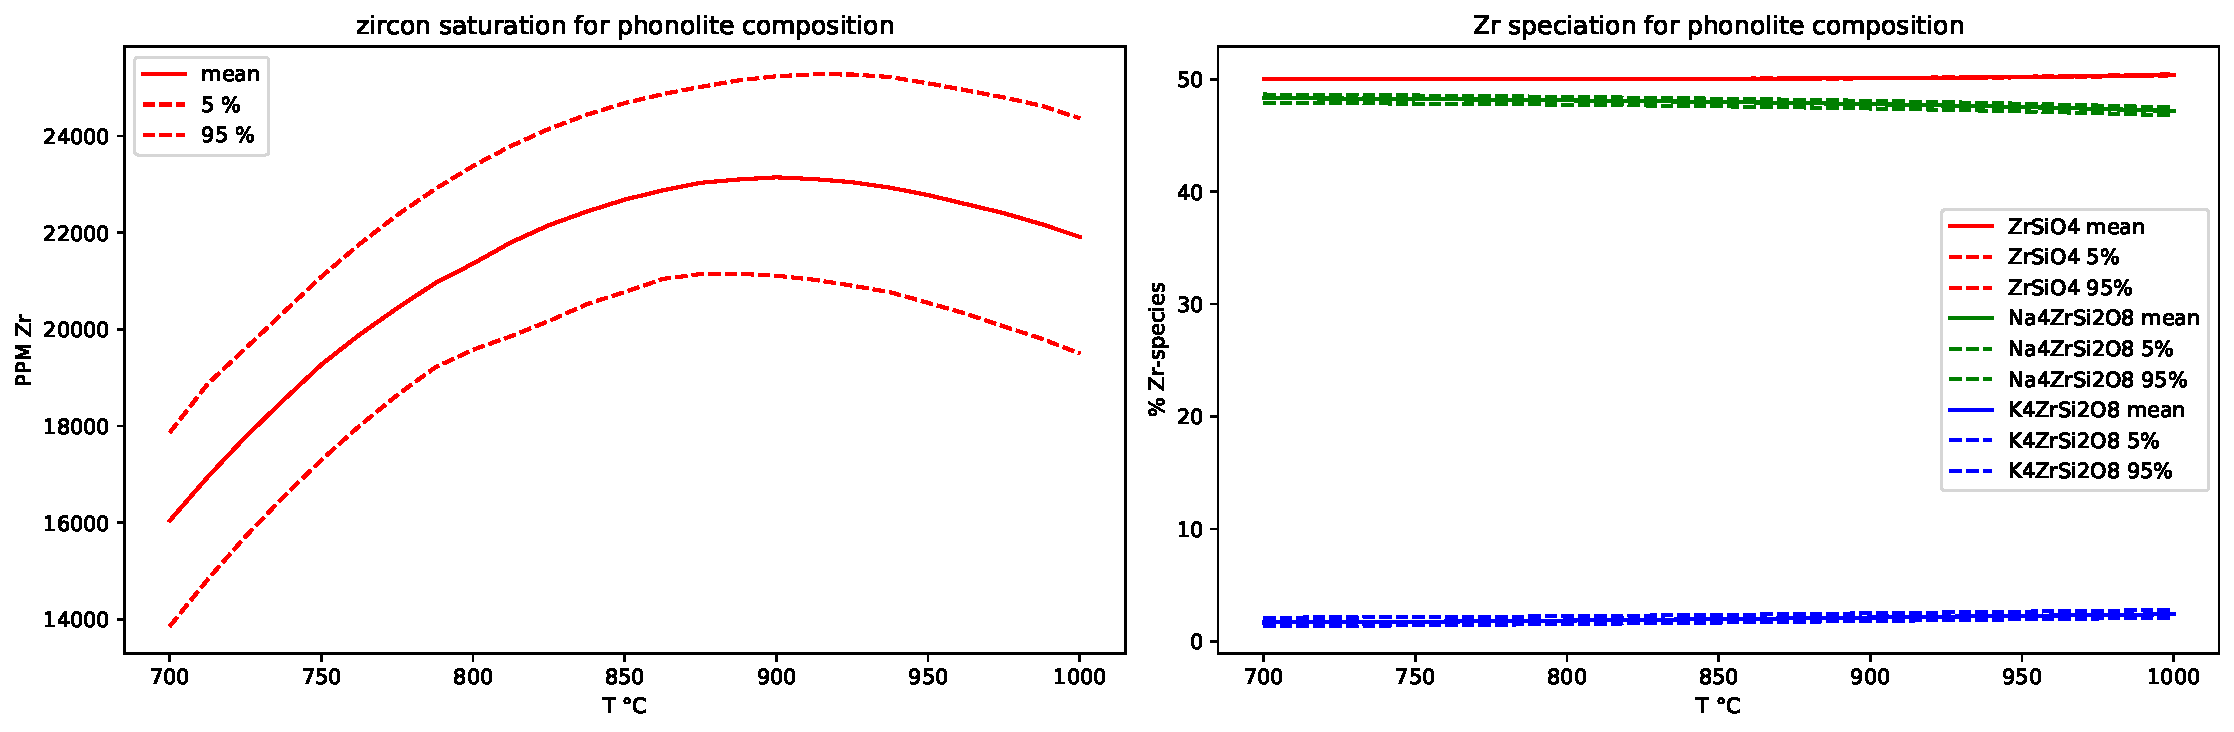
\includegraphics{images/zircon_sat_phonolite.pdf}

}

\subcaption{\label{fig-4h}Phonolite}

\end{minipage}%
\newline
\begin{minipage}{\linewidth}

\centering{

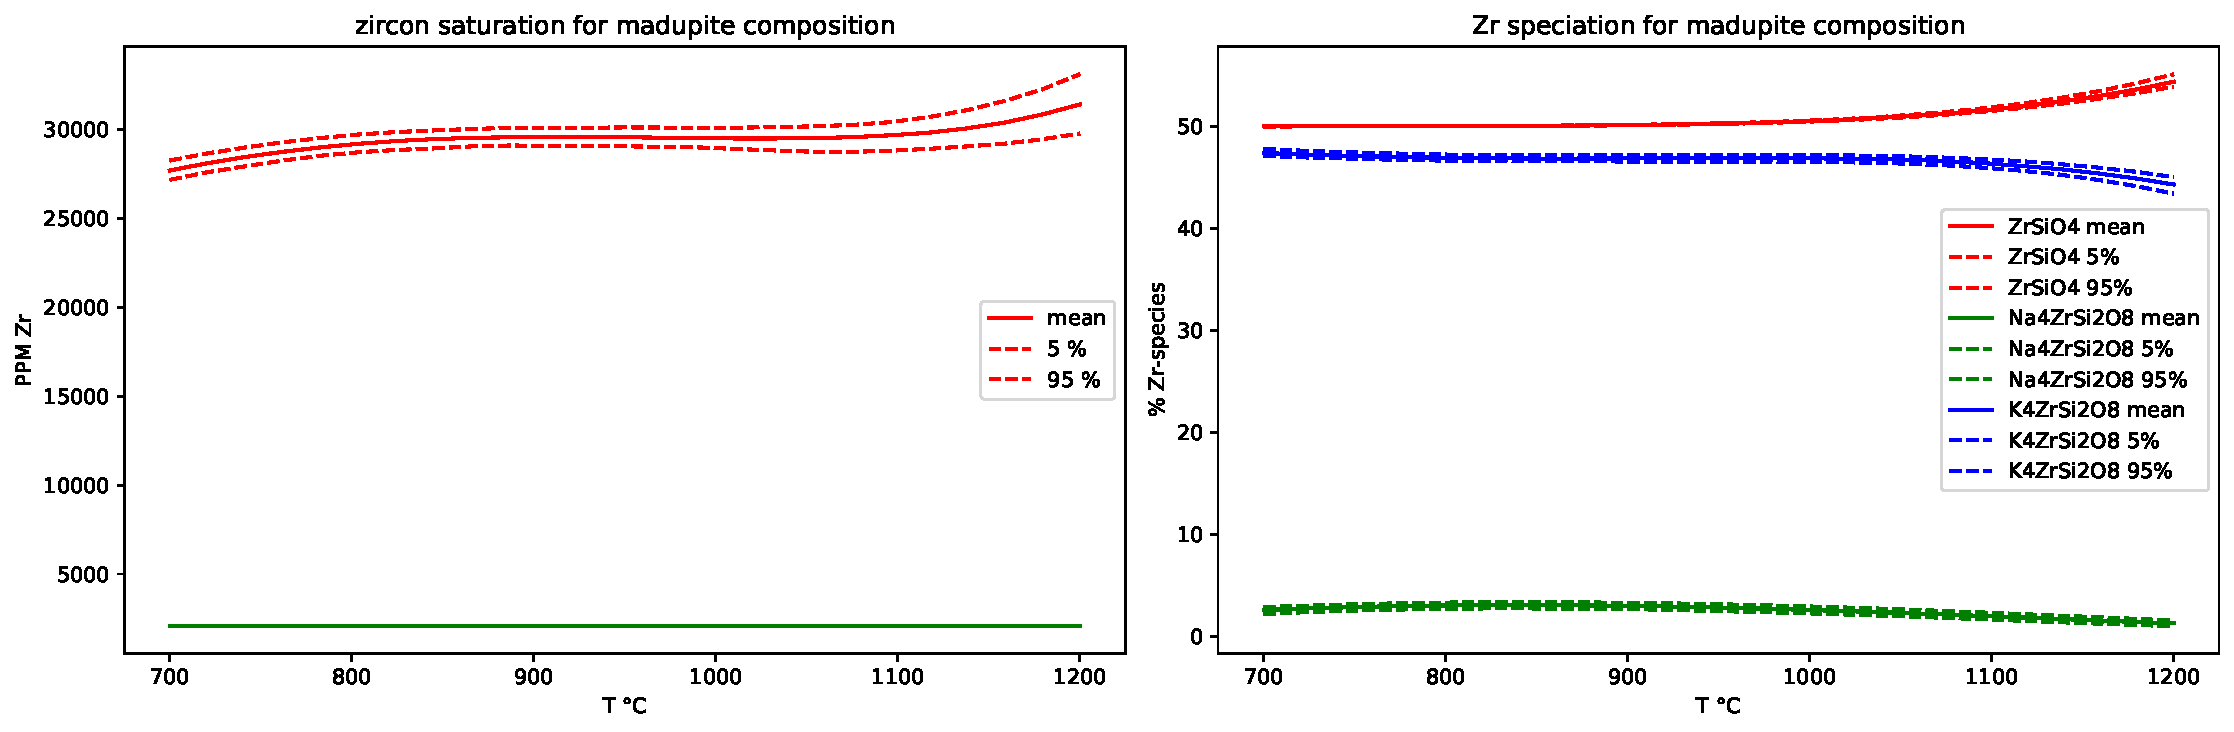
\includegraphics{images/zircon_sat_madupite.pdf}

}

\subcaption{\label{fig-4i}Madupite}

\end{minipage}%
\newline
\begin{minipage}{\linewidth}

\centering{

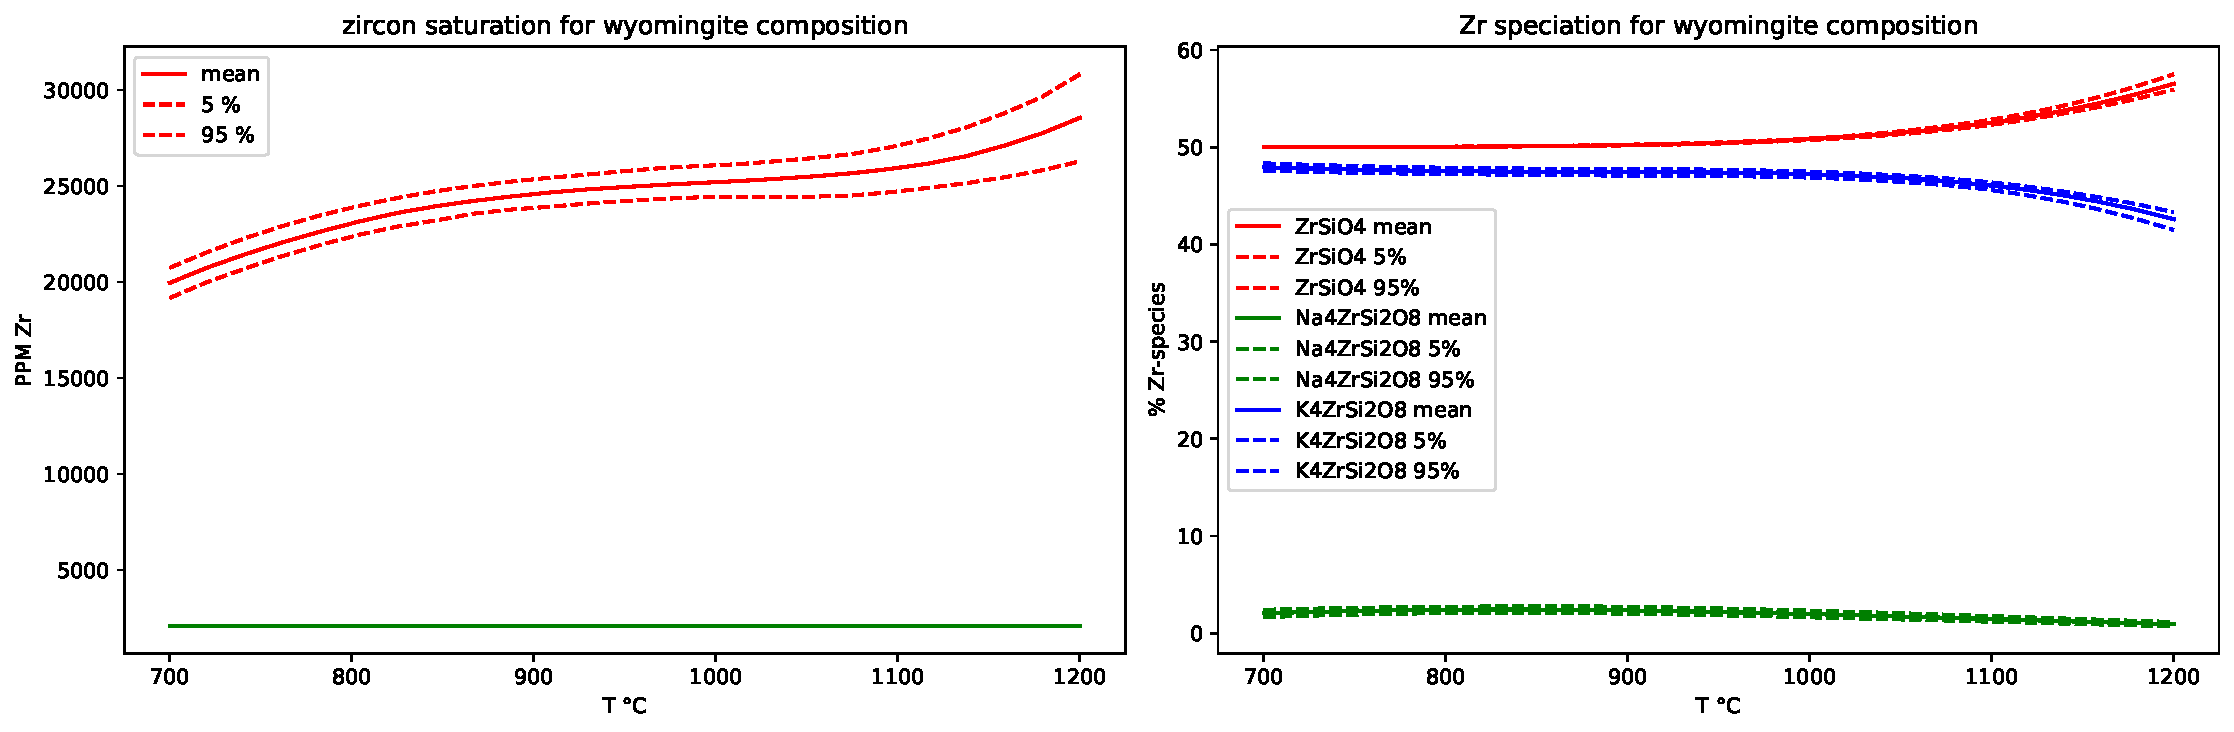
\includegraphics{images/zircon_sat_wyomingite.pdf}

}

\subcaption{\label{fig-4j}Wyomingite}

\end{minipage}%

\caption{\label{fig-4}Zircon Saturation Curves}

\end{figure}%

For each magma type listed in Table~\ref{tbl-4} a zircon saturation
curve is constructed and plotted in Figure~\ref{fig-4a} through
Figure~\ref{fig-4j}. For each sub-figure, the mean zircon saturation
curve is plotted along with its 5\% and 95\% quartile. Calculations are
based on a Monte Carlo propoagtion of uncertainties using parameter
estimates constructed from the variance-covariance matrix of
Table~\ref{tbl-3}. The right-most panels display abundances of
zirconium-bearing species in the melt with equivalent quartile
estimates.

At reported Zr concentrations, saturation conditions for fluid-saturated
high-silica rhyolite (Bishop Tuff, Figure~\ref{fig-4a}) are similar to
those estimated using the empirical geothermometer of Watson and
Harrison (1983). Saturation conditions for the Iceland rhyolite
(Thingmuli, Figure~\ref{fig-4b}) are consistent with expected
higher-temperatures of these lavas given their lower water contents. The
Iceland rhyolite also has a higher Na/K ratio than its continental
equivalent. The northern California rhyolite displayed in
Figure~\ref{fig-4c} has saturation conditions similar to the Bishop
magma, and the dacite (Figure~\ref{fig-4d}) is undersaturated with
zircon at the expected storage temperature conditions, but Zr contents
are consistent with saturation for a rhyolitic residuum of this bulk
composition.

Despite their high Zr-concentrations, peralkaline rhyolites in
Table~\ref{tbl-4} (a pantellerite from Pantelleria and a comendite from
Mayor Island, NZ) are not saturated with zircon. Water contents for the
pantellerite (Lowenstern and Mahood, 1991) are \textasciitilde1.8 wt\%
and consequently the inferred solidus temperatures are high, perhaps
comparable to Icelandic rhyolites. Reported Zr abundances in these lavas
(1800 and 2300 PPM, respectively) suggest model zircon saturation
temperature below \textasciitilde750°C (Figure~\ref{fig-4e}) and
\textasciitilde870°C (Figure~\ref{fig-4f}). Arguing from the basis of
phase relations for the ferromagesian silicates and the absence of Fe-Ti
oxides associated with these lavas, Nicholls \& Carmichael (1969)
conclude that likely liquidus temperatures fall between 900°C and
1025°C. Given that water contents of the magma indicate strongly
undersaturated conditions, the solidus is likely to be within 100°C of
liquidus. Our model predictions of zircon saturation are consistent with
these conclusions, indicating that Zr-concentration is barely sufficient
to saturate these lavas with zircon prior to eruption.

Model stauration curves for trachyte (Figure~\ref{fig-4g}) and phonolite
(Figure~\ref{fig-4h}) reveal that Zr-concentrations must be on the order
of a weight percent in order to saturate these liquids with zircon. An
additional observation is that the shape of the saturation curves is
strongly influenced by temperature. To understand why, consider that
these liquids simultaneously have higher absolute concentrations Zr and
Na and higher Na/K ratios; the Na-zirconate species has abundance
comparable to ZrSiO4. Assuming \(x\) is the fraction of Na-zirconate
species and \(1-x\) is the fraction of ZrSiO4, the dissolution of zircon
proceeds via the reaction:

ZrSiO4\emph{zircon} + \(2 x\) Na2SiO3\emph{liquid} = \(x\)
Na4ZrSi2O8\emph{liquid} + \(\left( 1-x \right)\) ZrSiO4\emph{liquid} +
\(x\) SiO2\emph{liquid}

The temperature dependence of zircon saturation is consequently a
reflection of the entropy of this dissolution reaction, which is

\begin{equation}\phantomsection\label{eq-9}{
\Delta S = x \bar{s}_{Na_4ZrSi_2O_8}^{liquid} + \left( 1-x \right) \bar{s}_{ZrSiO_4}^{liquid} + x \bar{s}_{SiO_2}^{liquid} - 2 x \bar{s}_{Na_2SiO_3}^{liquid} - \bar{s}_{ZrSiO_4}^{zircon}
}\end{equation}

The standard state entropy change contribution to Equation~\ref{eq-9} is
zero under the model calibration asumptions made previously, so, this
expression reduces to:

\begin{equation}\phantomsection\label{eq-10}{
\Delta S \approx - x R \log X_{Na_4ZrSi_2O_8} - \left( 1-x \right) R \log X_{ZrSiO_4} - x R \log X_{SiO_2} + 2 x R \log X_{Na_2SiO_3} \approx - R \log \left( \frac{X_{Na_4ZrSi_2O_8}^x X_{ZrSiO_4}^{1-x} X_{SiO_2}^x}{X_{Na_2SiO_3}^{2x}} \right) = - R \log \left( X_{Na_4ZrSi_2O_8}^x X_{ZrSiO_4}^{1-x} \right) - R x \log \left( \frac{X_{SiO_2}}{X_{Na_2SiO_3}^{2}} \right)
}\end{equation}

if we consider non-ideal contributions to the Gibbs Free Energy to be
second order. If \(z\) is the total mole fraction of all zirconate
species, then \(X_{Na_4ZrSi_2O_8}\) is approximately \(z x\) and
\(X_{ZrSiO_4}\) is approcimately \(z \left( 1-x \right)\), and
Equation~\ref{eq-10} becomes

\begin{equation}\phantomsection\label{eq-11}{
\Delta S \approx - R \log \left[ z^x x^x z^{1-x} \left( 1 - x \right) ^{1-x} \right] - R x \log \left( \frac{X_{SiO_2}}{X_{Na_2SiO_3}^{2}} \right) = -R \log z - R \left[ x^x \left( 1 - x \right) ^{1-x} \right] - R x \log \left( \frac{X_{SiO_2}}{X_{Na_2SiO_3}^{2}} \right)
}\end{equation}

The last logaithmic term in Equation~\ref{eq-11} is a linear function of
the fraction of Na-zirconate species (\(x\)) and for the trachyte bulk
composition is approximately \(- 41 x\) J. The first term has a value of
approximately 40 J, but decreases as Zr concentration in the melt
increases. The central term has a positive maximum at
\(x = \frac{1}{2}\) of \textasciitilde{} 6 J and falls parabolically to
zero at lower or higher Na-zirconate mole fractions.

This analysis allows us to better understand the shape of the zircon
saturation curves for the trachyte and phonolite. A positive slope for
these curves requires a positive \(\Delta S\), as the dissolution
reaction must go to the right as temperature increases, and in previous
cases, where the total mole fraction of Zr-bearing species in the liquid
is very low, the first term in Equation~\ref{eq-11} dominates and the
saturation curves have a positive slope. However, as the
Zr-concentration in the melt increases, the dominance of the first term
diminishes, the contribution of the second and third terms become
significant in determing the sign of the entropy change. In particular,
if the fraction of Na-zirconate species decreaes with increasing
\emph{T}, then the third term in Equation~\ref{eq-11}, which is
negative, is more likely to dominate the exression and lead to a
turnover in the saturation curve. The conclusion is that higher overall
concentration of Zr in the liquid coupled with the presence of near
equal abundances of Na-zirconate and ZrSiO4 species, governs the unusual
shape of the zircon saturation curves. If these magmas did saturate with
zircon, its presence would lead to an unsatisfactory geothermometer.

The final magma types considered, maduite (Figure~\ref{fig-4i}) and
wyomingite (Figure~\ref{fig-4j}), represent bulk compositions with
extremely high K/Na ratios. Neither magma precipitates zircon, but both
form a Zr-bearing phenocryst phase, wadeite. Reported concentrations of
Zr are at the 2000 PPM level. Our model calculations suggest that
measured concentrations are about an order of magnitude below those
required to saturate zircon, and that Zr is predominantly presence as
both K-zirconate and ZrSiO4 species in the melt.

The calculations summarized in Figure~\ref{fig-4a} through
Figure~\ref{fig-4j} were performed at a pressure of 200 MPa. The effect
of pressure on these results is insignificant, e.g.~for the high-silica
rhyolite assuming 100 PPM Zr in the liquid, the saturation temperature
is 744.7°C at 100 Ma, 745.5°C at 200 MPa, 745.9°C at 300 MPa. This
effect is typical for all compositions examined.

\subsection{Phase Equilibria}\label{phase-equilibria}

\begin{figure}

\centering{

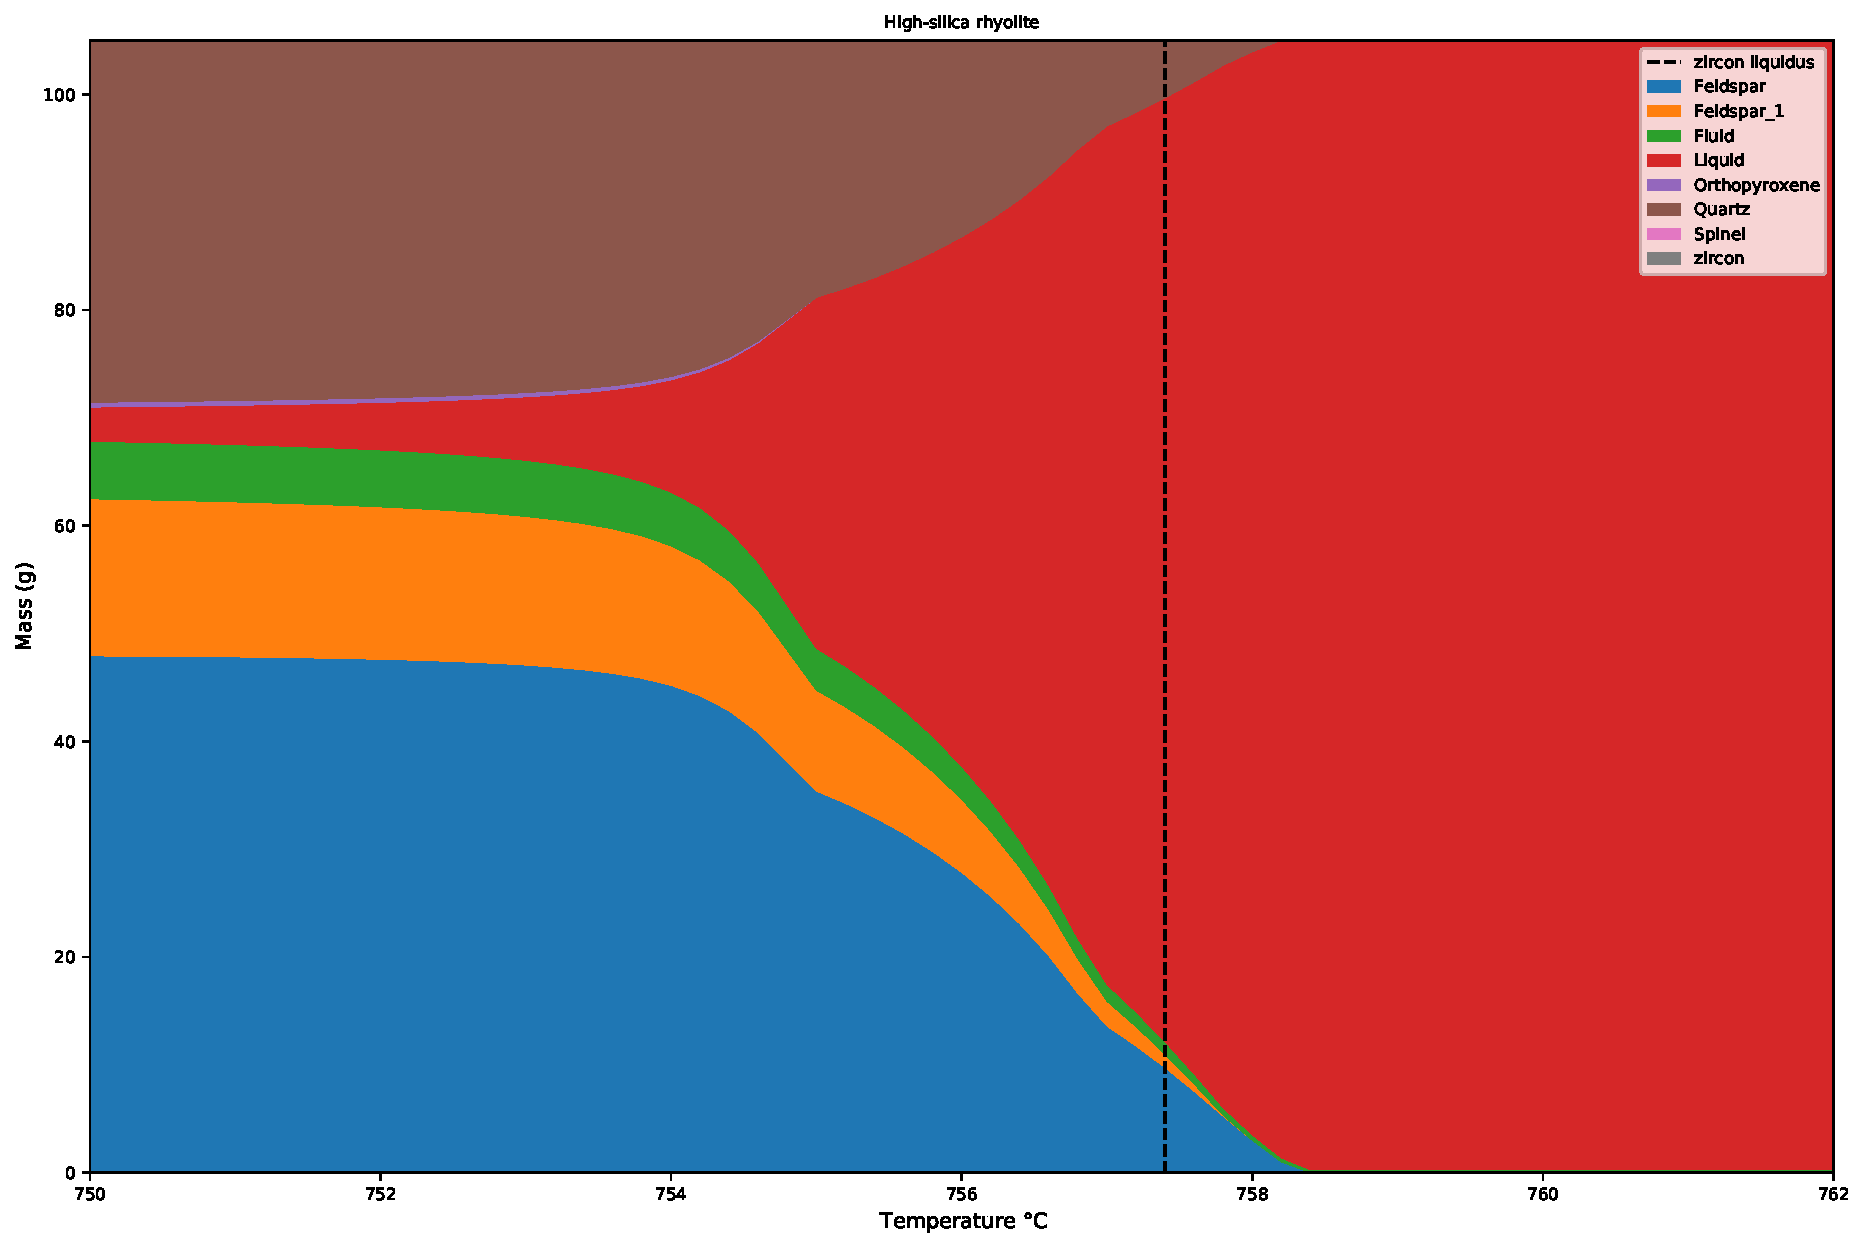
\includegraphics[width=1\textwidth,height=\textheight]{images/MELTS-zr-rhyolite.pdf}

}

\caption{\label{fig-5}Phase relations for high-silica rhyolite
calculated using rhyolite-MELTS (v1.1) and the model presented in this
paper. Equilibrium crystallization. Dashed line denotes the onset of
zircon saturation at 757.4°C.}

\end{figure}%

As the calibrated model is compatible with rhyolite-MELTS (v. 1.1), we
may use it to calculate phase equilibria in zircon-bearing assemblages.
In Figure~\ref{fig-5} phase proportions during crystallization of a
high-silica rhyolite (Table~\ref{tbl-4}) are illustrated. The workflow
for this calculation is documented in
\href{notebooks/7-MELTS-with-Zr.ipynb}{this Jupyter notebook}.

The most notable feature of the phase diagram presented in
Figure~\ref{fig-5} is that the onset of zircon saturation is at 757.4°C
in contrast to the calculated geothermometer temperature of 745.9°C (see
below). This temperature difference is due largely to the effect of
expulsion of fluid and the crystallization of two feldspars and quartz,
which elevates the concentration of the incompatible element Zr in the
liquid, permiting saturation of zircon at higher temperature. This
temperature discrepancy highlights the liklihood that application of
zircon geothermometry to bulk rock compositions is problematic, even
when such compositions are representitive of near eutectic melts. In
practical terms, the uncertainty in calculated phase relations is large
enough to encompass these temperature differences, but the relative
offset is important to consider, and every effort should be made to
utilize high quality glass analyses to avoid systematic bias.

\subsection{Geothermometry}\label{geothermometry}

\begin{figure}

\begin{minipage}{\linewidth}

\centering{

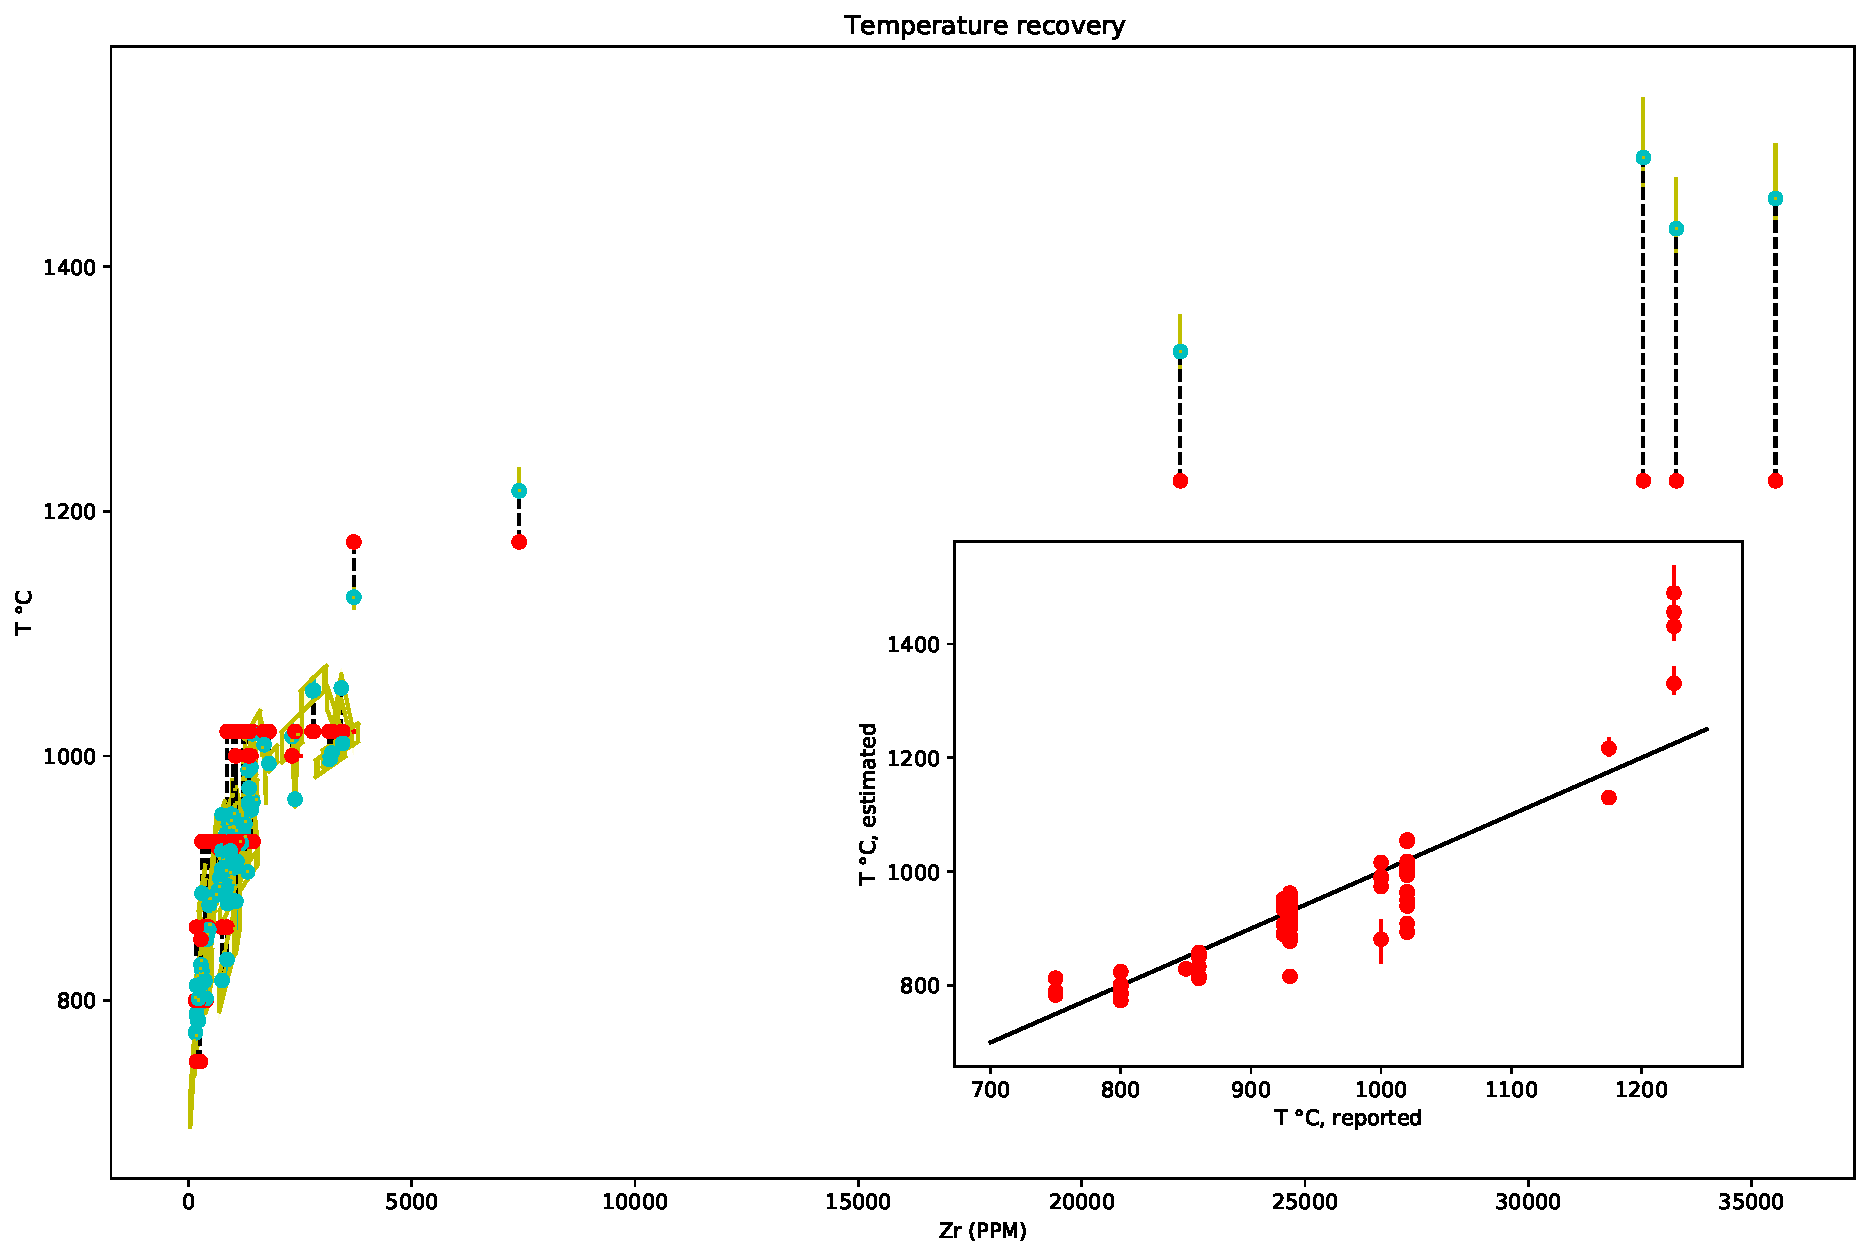
\includegraphics{images/Temperature_recovery.pdf}

}

\subcaption{\label{fig-6a}Temperature recovery for the calibration data
set. Red symbols denote reported temperatures and Zr concentration (with
uncertainties), green symbols the most likely model temperature. Each
green symbol is enclosed by a parallelogram (in yellow) whose vertices
are defined by the 5\% and 95\% quartiles associated with Monte Carlo
error propagation of model parameters. The reported and most likely
model temperature are connected by a black dashed line for each
expetimental datum. The inset plots reported temperature against model
temperature for the average Zr concentration with error brackets at the
5\% and 95\% quartile.}

\end{minipage}%
\newline
\begin{minipage}{\linewidth}

\centering{

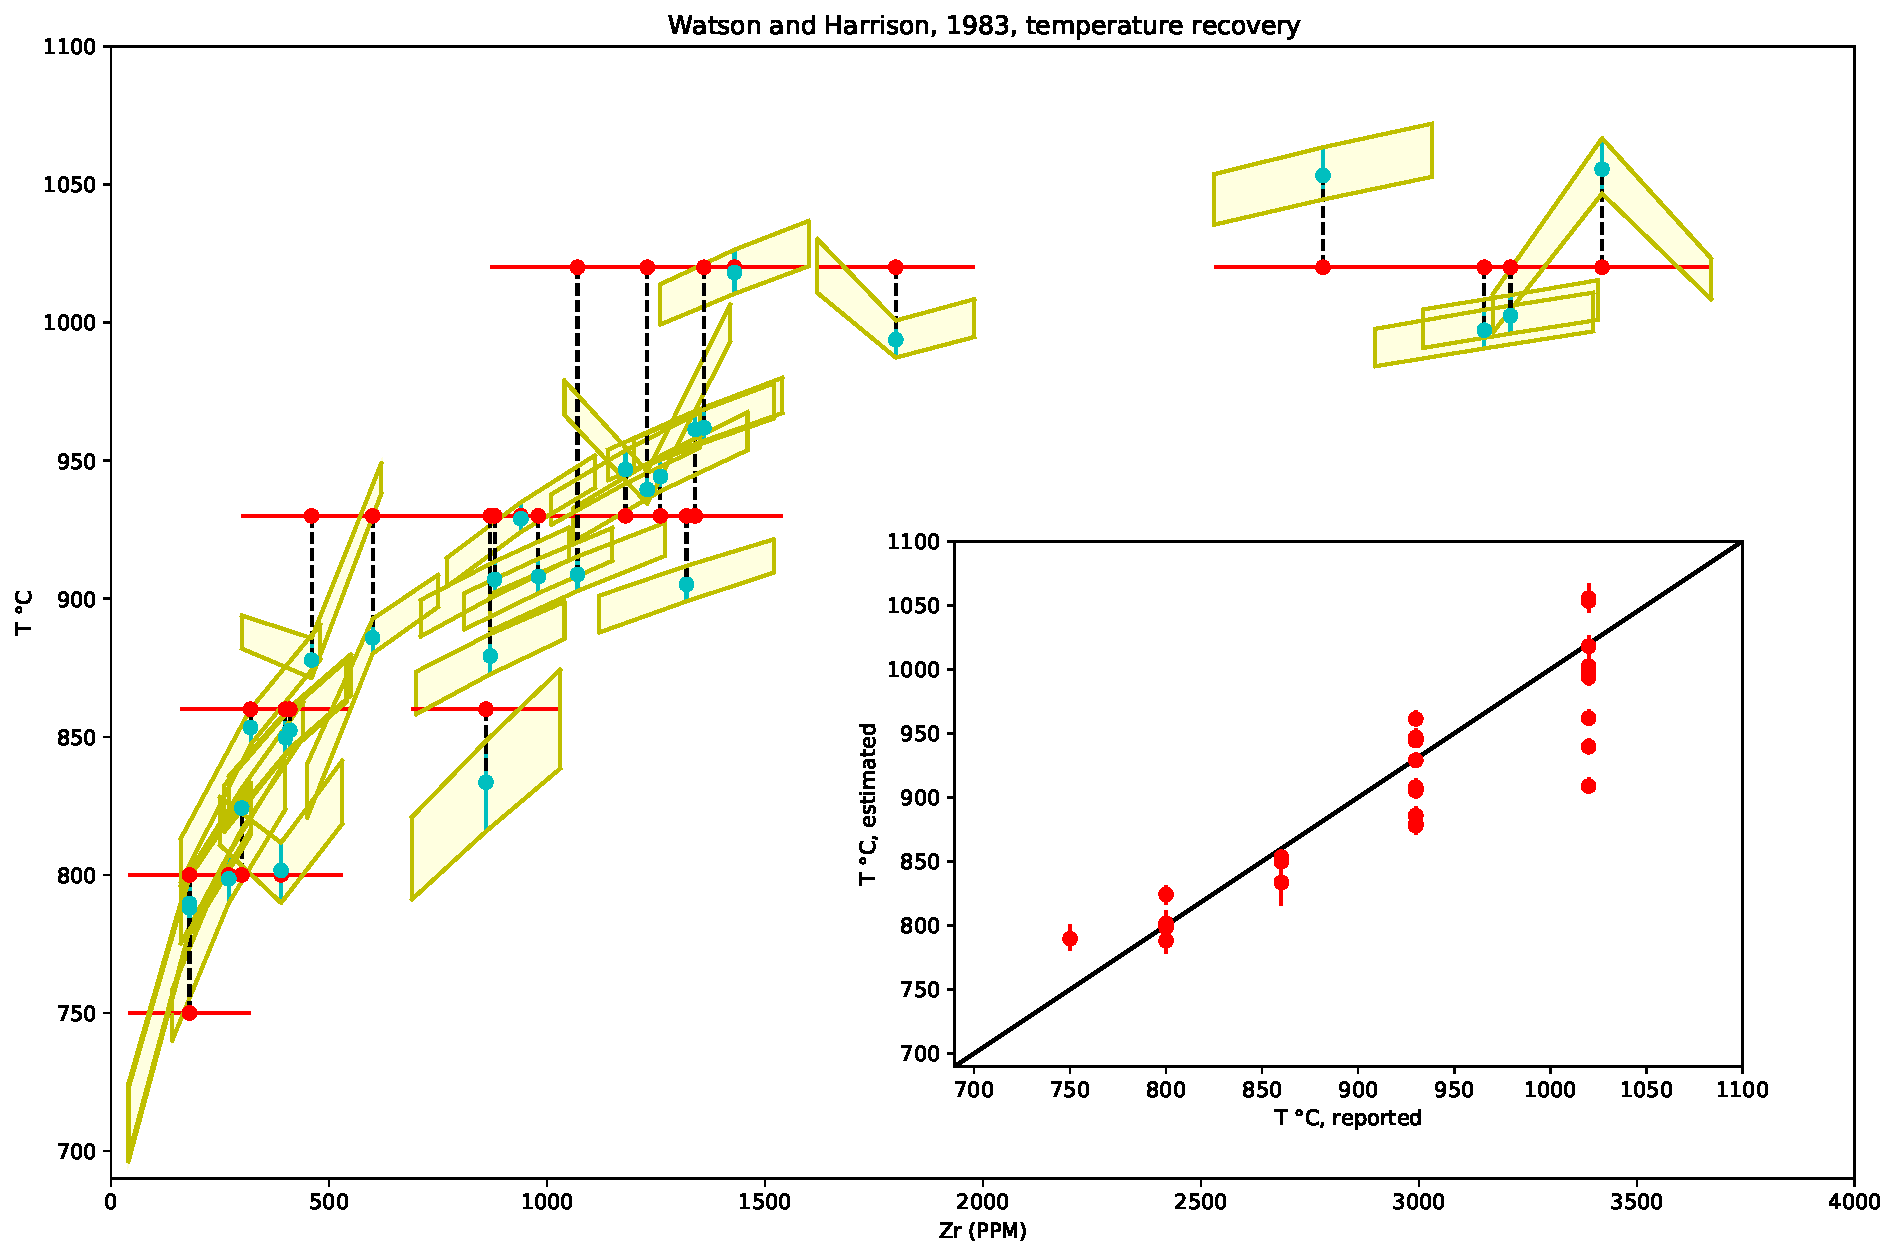
\includegraphics{images/WandH_1983_temperature_recovery.pdf}

}

\subcaption{\label{fig-6b}Temperature recovery for the E. Bruce Watson
\& Harrison (1983) data set. See legend for panel ``a''.}

\end{minipage}%
\newline
\begin{minipage}{\linewidth}

\centering{

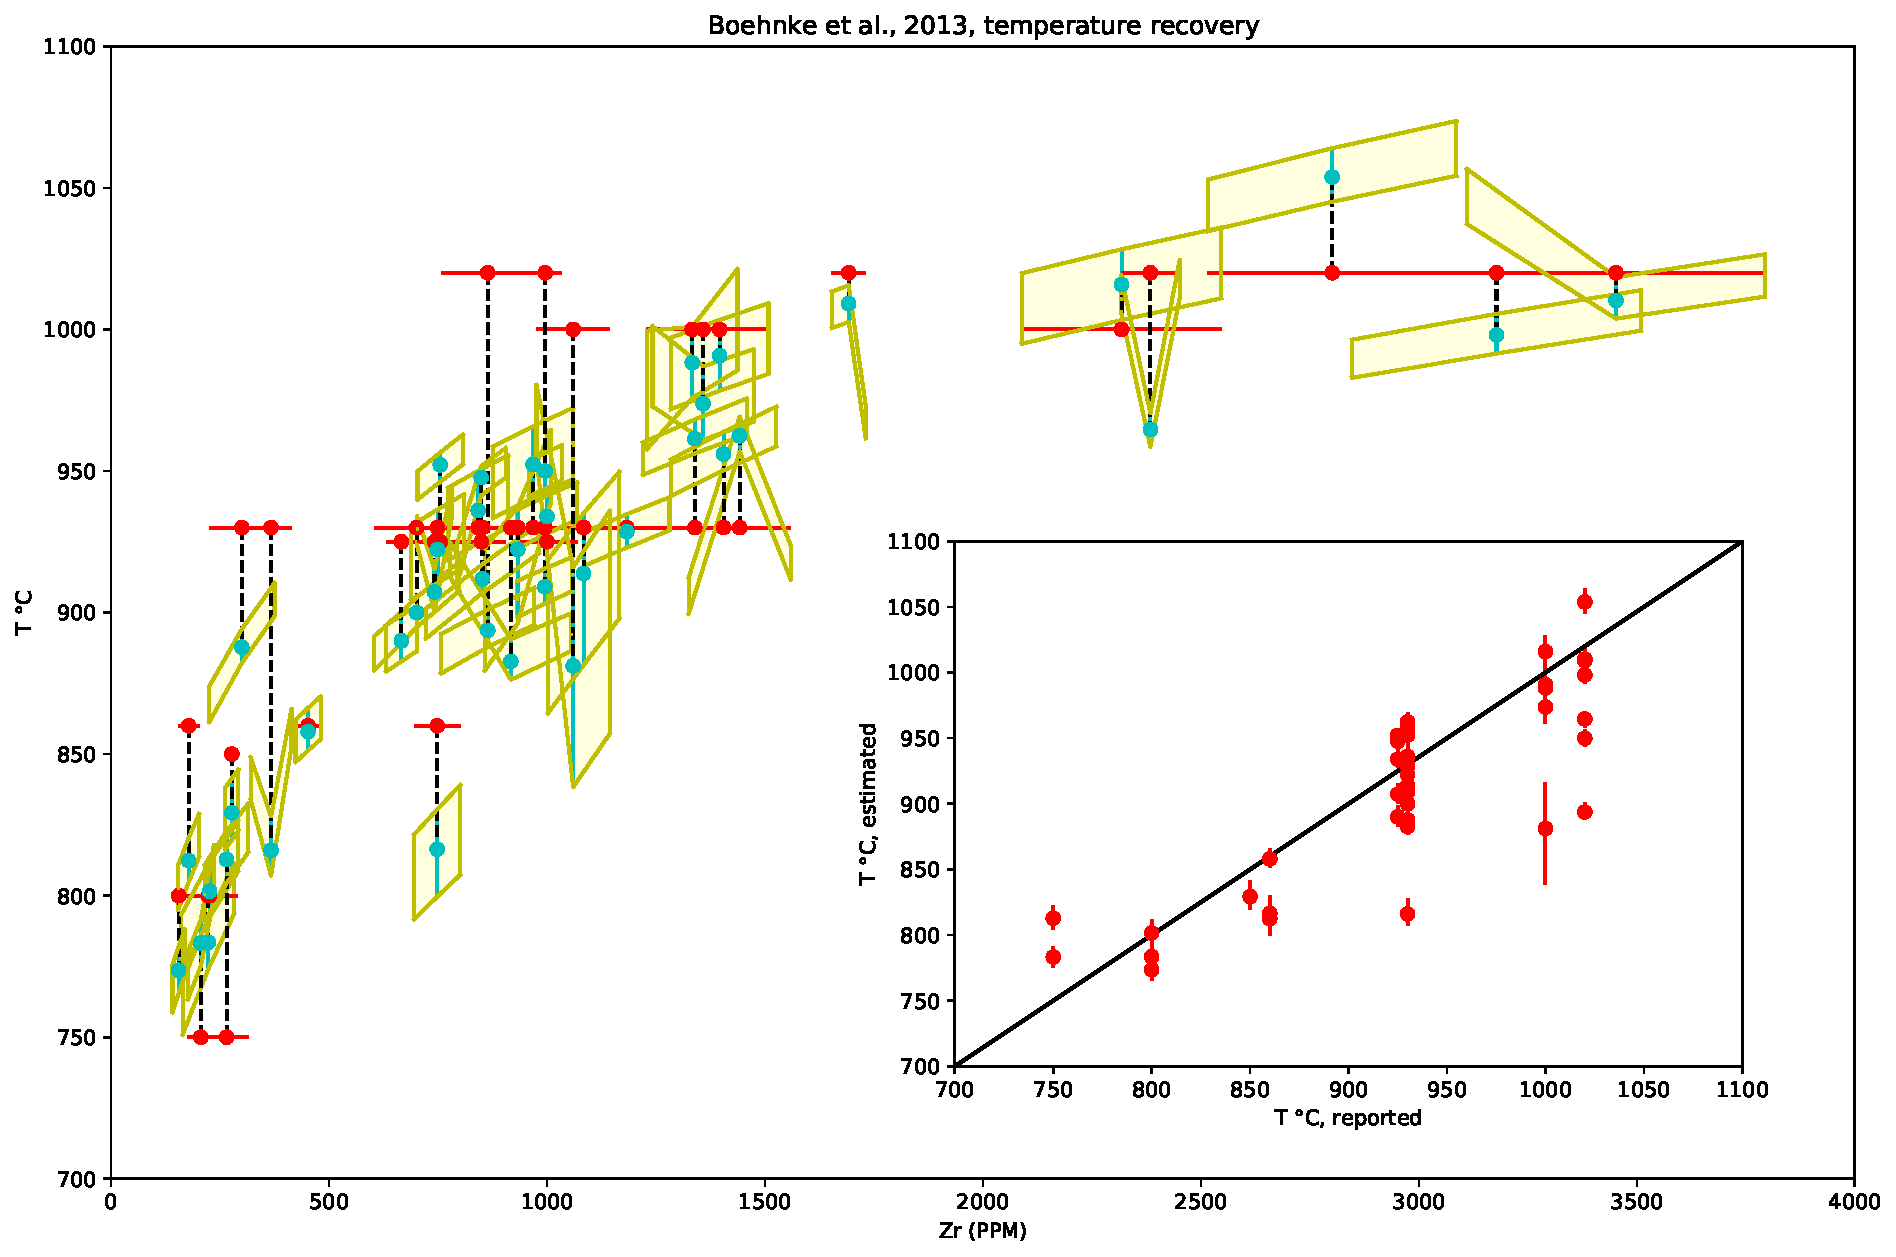
\includegraphics{images/Boehnke_2013_temperature_recovery.pdf}

}

\subcaption{\label{fig-6c}Temperature recovery for the Boehnke et al.
(2013) data set. See legend for panel ``a''.}

\end{minipage}%
\newline
\begin{minipage}{\linewidth}

\centering{

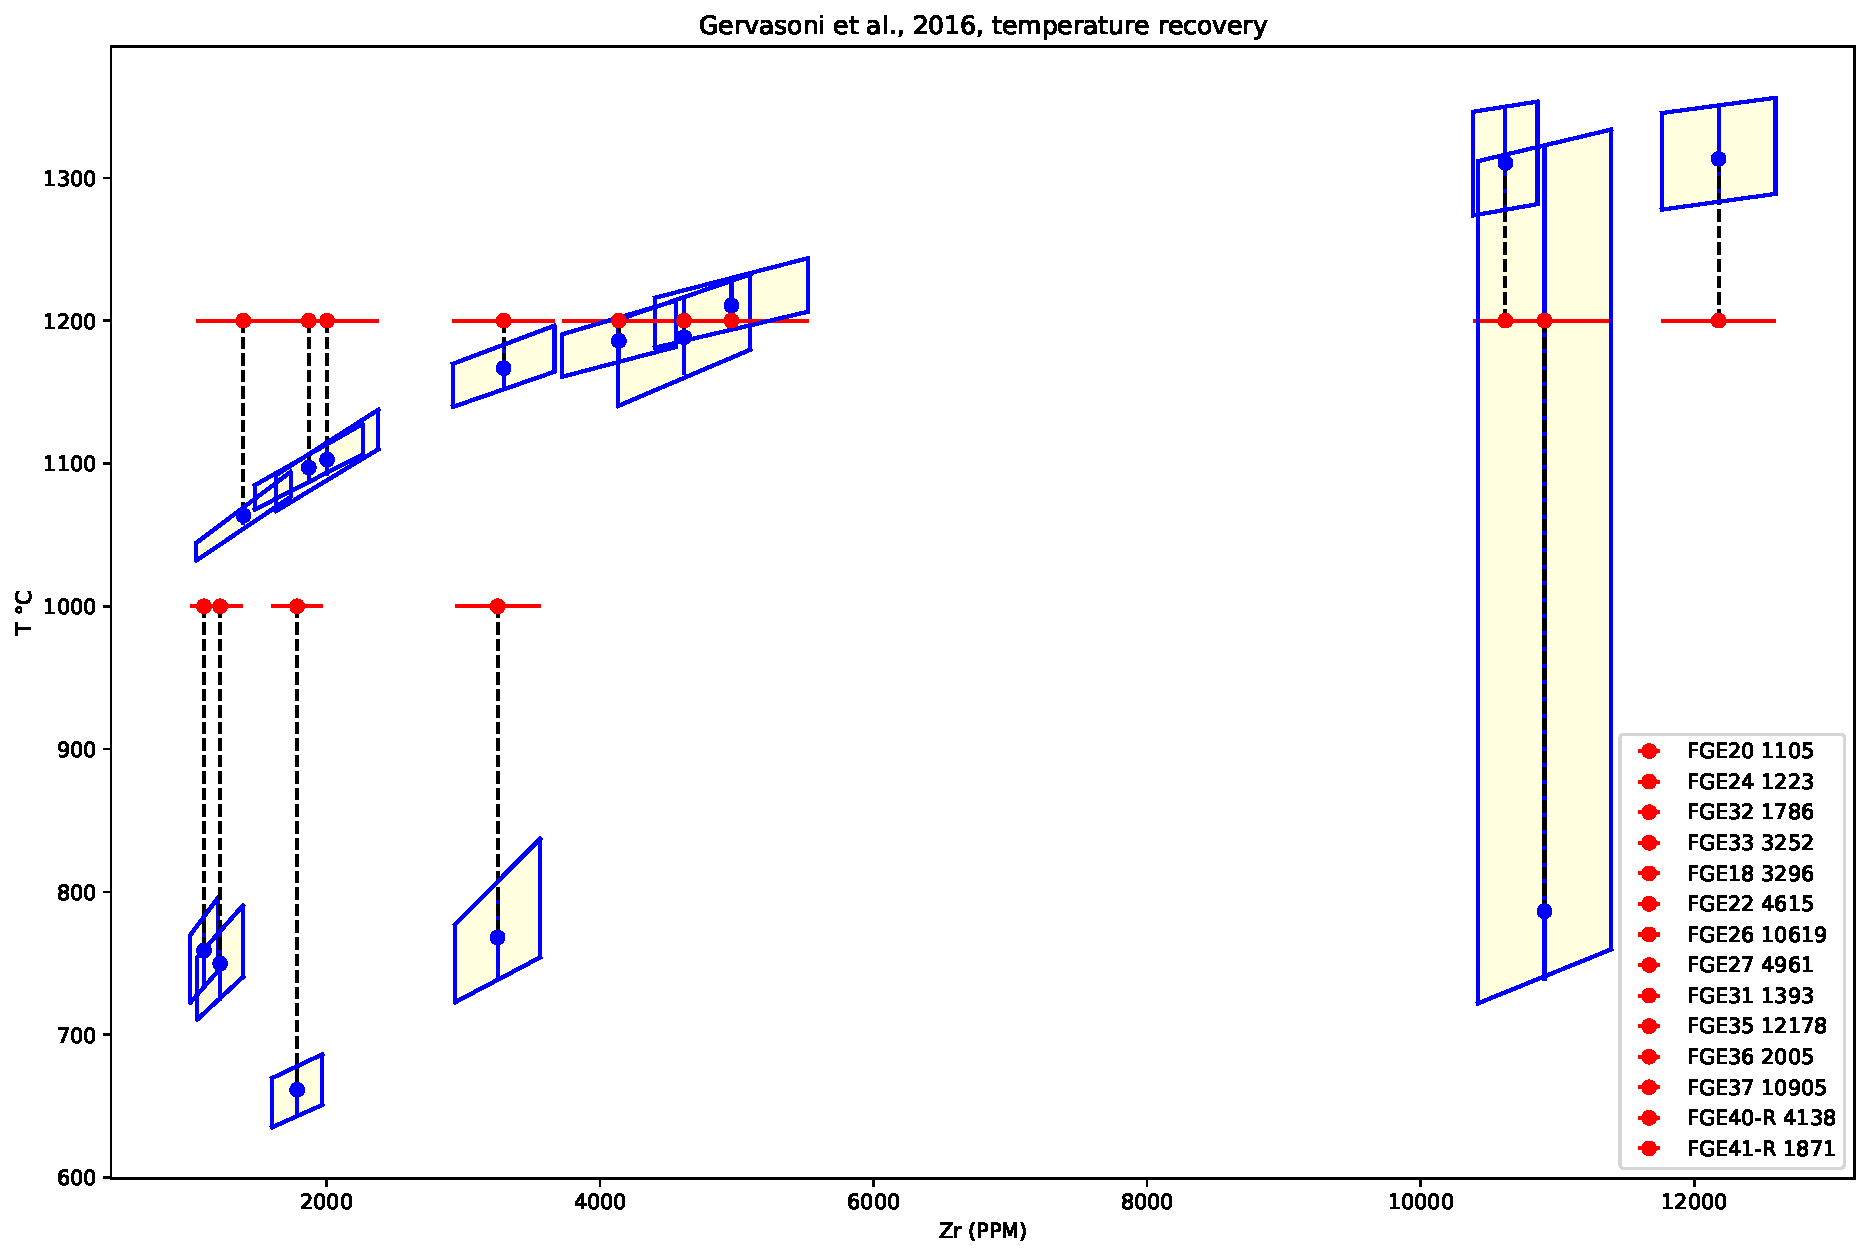
\includegraphics{images/Gervasoni_et_al.pdf}

}

\subcaption{\label{fig-6d}Temperature predictions for the Gervasoni et
al.~(2016) data set. Experiments are labeled, indicating Zr
concentration. Otherwsie, symbols are plotted as described for panel
``a''.}

\end{minipage}%

\caption{\label{fig-6}Temperature recovery from zircon saturation data
sets}

\end{figure}%

Software is available to utilize the model presented here as a
\href{notebooks/6-Liquid-MELTS-calib-2.ipynb}{geothermometer}. In
Figure~\ref{fig-6a} through Figure~\ref{fig-6d} we use this software to
calculate apparent experimental temperatures for the calibration data
set and for the data set of Gervasoni et al. (2016). These results
provide an alternative measure of how well the model recovers the
calibration data set, and suggests some potential problems with
attainment of equilibrium in the data set of Gervasoni.

Temperature estimates for the calibration data set are plotted in
Figure~\ref{fig-6a} with data from E. Bruce Watson \& Harrison (1983)
isolated in Figure~\ref{fig-6b} and selected low-Zr experiments from
Boehnke et al. (2013) displayed in Figure~\ref{fig-6c}. Experimental
values with uncertainties are plotted in red and temperature estimates
with model uncertainties are plotted as yellow polygons, with a green
dot at the most likely value. The inset on each panel shows model
temperture estimates with associated 5\% and 95\% quartiles, computed
using the average analytical Zr concentration, plotted against reported
experimental temperaure.

Model temperature estimates scatter about experimental temperatures for
Zr liquid concentrations below 4000 PPM. Above that concentration, the
model tends to overestimate temperature. This failure is probably
related to our model formulation assumption that regular solution
interaction parameters involving Zr-species are zero, implicitely
rendering the model applicable to a Henrian concentration limit. This
assumption could be relaxed in order to accomodate these data, but there
are so few data points at higher Zr-concentrations available for
calibration that the danger of overfitting does not warrant this
extension. Model error in temperature estimates due to parameter error
propagation is -7.3°C, +8.1°C (5\%, 95\%) for the E. Bruce Watson \&
Harrison (1983) data set (Figure~\ref{fig-6b}), with the average error
in recovered experimental temperature of -14°C (± 35°C). Including
measured uncertainty in Zr concentration brings the average recovered
temperature within the range -34°C (Zr - 2 sigma) to 4°C (Zr + 2 sigma)
with the standard deviation of the low and high estimates maintained at
the same level as the average Zr value. For the Boehnke et al. (2013)
data set (Figure~\ref{fig-6c}, ignoring the 4 data points above 4000 PPM
Zr), the recovery of temperature estimates due to parameter error
propagation is -11.6°C, +10.1°C (5\%, 95\%). The average error in
recovered experimental temperature is -15°C (± 41°C) with the range
-17°C ± 35°C (Zr - 2 sigma) to -5°C ± 39°C (Zr + 2 sigma).

Temperature recovery of the data set of Gervasoni et al. (2016), which
was not used in calibration, is shwon in Figure~\ref{fig-6c}. Note that
model temperatures are overestimated for glass compositions with
\textgreater{} 6000 PPM Zr, as found with the data set of Boehnke et al.
(2013). At experimental temperatures of 1200°C at at Zr concentrations
\textgreater{} 2500 PPM and \textless{} 6000 PPM, temperature recovery
is comparable to the calibration data sets. At lower Zr concentrations
and at lower temperatures, temperature recovery is systematically
biased. The experimental data set of Gervasoni et al. (2016) differes
from the calibration data sets in showing almost complete iron-loss to
the experimental capsule. In addition, these experiments were conducted
under nominally dry conditions (unlike the other two studies) and run
durations were realtively short (24 hrs). Considering the absence of
volatiles, which would aid reaction kinetics, all these factors support
our contention that equilibrium was not achieved in the lower
temperature, lower Zr-content runs. In fact, the partial agreement at
1200°C for the subset of ``intermediate'' Zr concentration experiments
may simply be fortuitous.

\section{Model Access}\label{model-access}

The model and dependent calculations presented here can be replicated in
full utilizing the associated Jupyter notebooks:
\href{notebooks/1-Model-description.ipynb}{Model-description},
\href{notebooks/2-Endmembers-MELTS.ipynb}{Endmembers},\href{notebooks/3-Liquid-MELTS-codegen.ipynb}{Solution
Model}, \href{notebooks/4-Liquid-MELTS-API-tests.ipynb}{Model Testing},
\href{notebooks/5-Liquid-MELTS-calib-1.ipynb}{Calibration 1},
\href{notebooks/6-Liquid-MELTS-calib-2.ipynb}{Calibration 2}, and
\href{notebooks/7-MELTS-with-Zr.ipynb}{MELTS with Zr}. These notebooks
will execute on an \href{http://enki-portal.org/index.html}{ENKI enabled
server platform} or, more conveniently, within a containerized image
implementation of the ThermoEngine software ecosystem (the ENKI software
engine) that may be downloaded from GitLab's Docker image
\href{https://gitlab.com/ENKI-portal/ThermoEngine}{containier
repository}. The container will execute on any computer that has a
recent version of \href{https://www.docker.com}{Docker} installed.

\section{Conclusions}\label{conclusions}

This paper updates MELTS (v 1.1) to account for phase relations
involving the trace element Zr. The saturation surface for zircon is
calibrated using experimental data from E. Bruce Watson \& Harrison
(1983) and Boehnke et al. (2013). The model is formulated and optimized
for Zr melt concentrations in the effective Henrian limit (\textless{}
4000 PPM) and accounts for the effect of alkalis on zircon saturation
via the adoption of an associated solution formulation that incorporates
three Zr-bearing melt species: ZrSiO4, Na4ZrSi2O8, and K4ZrSi2O8. The
model may be used (1) to calculate zircon phase relations in magmatic
composition melts, (2) to construct zircon saturation diagrams for a
given liquid bulk composition, and (3) as a geothermometer for zircon
bearing igneous rocks.

\section{Aknowledgements}\label{aknowledgements}

MSG is grateful to the extended MESSY group at Vanderbilt University for
suggesting this problem and for assisting in working through model
assumptions and calibration data sets. MSG also acknowledges material
support from NSF 17-25425 and from OFM Research.

\phantomsection\label{refs}
\begin{CSLReferences}{1}{0}
\bibitem[\citeproctext]{ref-boehnke2013zircon}
Boehnke, P., Watson, E. B., Trail, D., Harrison, T. M., \& Schmitt, A.
K. (2013). Zircon saturation re-revisited. \emph{Chemical Geology},
\emph{351}, 324--334.

\bibitem[\citeproctext]{ref-carmichael1967mineralogy}
Carmichael, I. S. (1967). The mineralogy and petrology of the volcanic
rocks from the leucite hills, wyoming. \emph{Contributions to Mineralogy
and Petrology}, \emph{15}(1), 24--66.

\bibitem[\citeproctext]{ref-carmichael1974igneous}
Carmichael, I. S., Turner, F. J., \& Verhoogen, J. (1974). \emph{Igneous
petrology}. New York, McGraw-Hill.

\bibitem[\citeproctext]{ref-gervasoni2016zircon}
Gervasoni, F., Klemme, S., Rocha-Júnior, E. R., \& Berndt, J. (2016).
Zircon saturation in silicate melts: A new and improved model for
aluminous and alkaline melts. \emph{Contributions to Mineralogy and
Petrology}, \emph{171}(3), 21.

\bibitem[\citeproctext]{ref-ghiorso2015h}
Ghiorso, M. S., \& Gualda, G. A. (2015). An H2O--CO2 mixed fluid
saturation model compatible with rhyolite-MELTS. \emph{Contributions to
Mineralogy and Petrology}, \emph{169}(6), 53.

\bibitem[\citeproctext]{ref-ghiorso1995chemical}
Ghiorso, M. S., \& Sack, R. O. (1995). Chemical mass transfer in
magmatic processes IV. A revised and internally consistent thermodynamic
model for the interpolation and extrapolation of liquid-solid equilibria
in magmatic systems at elevated temperatures and pressures.
\emph{Contributions to Mineralogy and Petrology}, \emph{119}(2-3),
197--212.

\bibitem[\citeproctext]{ref-ghiorso1983gibbs}
Ghiorso, M. S., Carmichael, I. S., Rivers, M. L., \& Sack, R. O. (1983).
The gibbs free energy of mixing of natural silicate liquids; an expanded
regular solution approximation for the calculation of magmatic intensive
variables. \emph{Contributions to Mineralogy and Petrology},
\emph{84}(2-3), 107--145.

\bibitem[\citeproctext]{ref-gualda2012rhyolite}
Gualda, G. A., Ghiorso, M. S., Lemons, R. V., \& Carley, T. L. (2012).
Rhyolite-MELTS: A modified calibration of MELTS optimized for
silica-rich, fluid-bearing magmatic systems. \emph{Journal of
Petrology}, \emph{53}(5), 875--890.

\bibitem[\citeproctext]{ref-linthout1984alkali}
Linthout, K. (1984). Alkali-zirconosilicates in peralkaline rocks.
\emph{Contributions to Mineralogy and Petrology}, \emph{86}(2),
155--158.

\bibitem[\citeproctext]{ref-lowenstern1991new}
Lowenstern, J. B., \& Mahood, G. A. (1991). New data on magmatic h 2 o
contents of pantellerites, with implications for petrogenesis and
eruptive dynamics at pantelleria. \emph{Bulletin of Volcanology},
\emph{54}(1), 78--83.

\bibitem[\citeproctext]{ref-nicholls1969peralkaline}
Nicholls, J., \& Carmichael, I. (1969). Peralkaline acid liquids: A
petrological study. \emph{Contributions to Mineralogy and Petrology},
\emph{20}(3), 268--294.

\bibitem[\citeproctext]{ref-Putirka_2008}
Putirka, K. D. (2008). {Thermometers and Barometers for Volcanic
Systems}. In Putirka, KD and Tepley, FJ (Ed.), \emph{{MINERALS,
INCLUSIONS AND VOLCANIC PROCESSES}} (Vol. 69, pp. 61--120). {Amer
Geophys Union; Mineralog Soc Amer; Dept Energy}.
\url{https://doi.org/\%7B10.2138/rmg.2008.69.3\%7D}

\bibitem[\citeproctext]{ref-robie1995thermodynamic}
Robie, R. A., \& Hemingway, B. S. (1995). \emph{Thermodynamic properties
of minerals and related substances at 298.15 k and 1 bar (105 pascals)
pressure and at higher temperatures} (Vol. 2131). US Government Printing
Office.

\bibitem[\citeproctext]{ref-seabold2010statsmodels}
Seabold, S., \& Perktold, J. (2010). Statsmodels: Econometric and
statistical modeling with python. In \emph{9th python in science
conference}.

\bibitem[\citeproctext]{ref-2020SciPy-NMeth}
Virtanen, P., Gommers, R., Oliphant, T. E., Haberland, M., Reddy, T.,
Cournapeau, D., et al. (2020). {{SciPy} 1.0: Fundamental Algorithms for
Scientific Computing in Python}. \emph{Nature Methods}, \emph{17},
261--272. \url{https://doi.org/10.1038/s41592-019-0686-2}

\bibitem[\citeproctext]{ref-watson1979zircon}
Watson, E. Bruce. (1979). Zircon saturation in felsic liquids:
Experimental results and applications to trace element geochemistry.
\emph{Contributions to Mineralogy and Petrology}, \emph{70}(4),
407--419.

\bibitem[\citeproctext]{ref-WATSON1983295}
Watson, E. Bruce, \& Harrison, T. M. (1983). Zircon saturation
revisited: Temperature and composition effects in a variety of crustal
magma types. \emph{Earth and Planetary Science Letters}, \emph{64}(2),
295--304.
https://doi.org/\url{https://doi.org/10.1016/0012-821X(83)90211-X}

\end{CSLReferences}



\end{document}
